% IMPORTANT: Please write various parts in different files, and then include
% them into this document.
% If you have a file called intro.tex then write: \include{intro}
% This is to avoid nasty merge conflicts, as well as to keep it tidy,
% modular, etc

\documentclass[11pt,a4paper,oneside]{report}


% Make bibliography appear in table of contents
\usepackage[nottoc,numbib]{tocbibind}

\usepackage{amsmath,amssymb,calc,ifthen,capt-of}


\usepackage[ampersand]{easylist}

% Allows us to click on links and references!
% http://tex.stackexchange.com/questions/73862/how-can-i-make-a-clickable-table-of-contents
\usepackage{hyperref}
\hypersetup{
    colorlinks,
    citecolor=black,
    filecolor=black,
    linkcolor=black,
    urlcolor=black
}

% Nice package for plotting graphs
% See excellent guide:
% http://www.tug.org/TUGboat/tb31-1/tb97wright-pgfplots.pdf
\usepackage{pgfplots}
\usepackage{amsmath,graphicx}
\usepackage{epstopdf}

\pgfplotsset{compat = newest}

% highlight - useful for TODOs and similar
\usepackage{color}
\newcommand{\hilight}[1]{\colorbox{yellow}{#1}}


\title{Attractor Neural Networks for Modelling Associative Memory}
\date{January 2013}
\author{
  Wael Al Jishi\\
  \texttt{wa910@imparial.ac.uk}
  \and
  Niklas Hambuechen\\
  \texttt{nh910@imparial.ac.uk}
  \and
  Razvan Marinescu\\
  \texttt{rvm10@imperial.ac.uk}
  \and
  Mihaela Rosca\\
  \texttt{mcr10@imparial.ac.uk}
  \and
  Lukasz Severyn\\
  \texttt{lk1110@imparial.ac.uk}
}


\begin{document}
\belowdisplayskip=12pt plus 3pt minus 9pt
\belowdisplayshortskip=7pt plus 3pt minus 4pt
% General notes:

% Report Guidelines:
% http://www.doc.ic.ac.uk/lab/thirdyear/group-project/ReportGuidelines2012.pdf

% "This is more marketing than engineering. We don't want a diary"

% Tony: "How long? I don't know. Keep it short. 30 pages is absolutely fine.
% 40 a bit too much. 20 is a bit..."
% NOTE this excludes the appendices

% Keep it simple and to the point. Don't waffle

% Report is read by people who DONT know your work, though they are
% technically minded


\maketitle{}


\renewcommand{\abstractname}{Executive Summary}

\begin{abstract}
% Compulsory
% 1 page max. Tony: "third to half a page ideal probably"
% Anandha: "Don't put a photo of your group in the executive summary or
% something like that!"
% Wael: I would say it might be appropriate to do something like that in the
% presentation though. We can discuss and see.

Attractor Neural networks have been a subject of intensive research in the past 30 years. They have been proposed as a model of associative memory and have been used in ranging from facial and speech recognition to modelling biological activities of the human brain.


The aim of our project was to attain a deeper understanding of these networks by running various simulations and investigating their properties. For this purpose, we have demonstrated their importance by implementing an image recognition software. Furthermore, we have also used them as an aid for modelling a psychological concept known as Attachment Theory, in order to better understand the human mind and how to cure various mental disorders.


Our project attempts to model, at a metaphorical level, an individual's emotional mindset, and how it is formed due to the influences of experiences, which manifest as memories, encountered in early life. We have implemented several mathematical models of neural networks, that can simulate various functions of the brain. Amongst these, two of them are of uttermost importance: learning and recalling information.


We have used our networks to analyse and quantify the influence of memories, analysing factors affecting their probability of being recalled, or how they can be either forgotten or reinforced. The latter is extremely important for the psychological studies, since it paves the way for curing some mental disorders whose roots lie in negative experiences encountered early in life.

% should we include some of the results as well?
\end{abstract}


\tableofcontents

% Chapter 1
\chapter{Introduction}
% Tony: "1, 2, 3 pages"
% What is the problem?
% Why is it interesting?
% How did you solve it?
% How far did you get?

% Includes motivation, objectives, and contributions (what you achieved)
\section{Motivation}

%Understanding the human brain
The human brain is considered to be one of the most complex objects which have puzzled scientists and philosophers alike throughout the centuries. To gain an understanding of how this mysterious black box works, through experimentation and modelling, would be of great aid to the furthering of science and humanity alike. A part of this includes developing cures for a multitude of mental and brain-related disorders.

%Artificial neural networks
Several medical discoveries from the 20th century have enlightened our knowledge of the human brain. One consequence of this was the development of different mathematical models of artificial neural networks, inspired by the fields of biology and medicine.

% modelling the Attachment Theory. Watch out between the distinction between Self-Attachment and Attachment Theory
Our motivation is to use some of these neural networks to explore the mathematics of a developing theory called Self-Attachment. Part of Attachment theory, this strategy aims to help cure various mental problems that people currently facing. Recent research has shown that a mathematical methodology of analysing these disorders is starting to become feasible. \cite{net_model_neuroses}

The subsequent chapters will introduce the Attachment Theory and the mathematical model. We have mainly focused on the technical side, and have described psychological analogies that place our technical results in context of the theory.

\section{Objectives}

%Main Objectives
Our main objective is to confirm the results of previous work done by Federico Mancinelli, who has been analysing the attachment theory using neural networks. He has performed several experiments regarding clusters of attractors, basin sizes, and Gaussian-distributed patterns. Furthermore, we have been aiming at extending his results by exploring the following concepts:
\begin{itemize}
\item Using the network for performing image recognition
\item Restricted Boltzmann machines
\item Super-attractors
\end{itemize}

%Improvement of Federico's results
In addition to that, we were aiming to improve some of the methods that were used in his experiments. This includes the technique for sampling Gaussian-distributed patterns or for calculating basin sizes. Our final aims consisted of explaining some of the subsequent inconsistencies that have been found in his results.

\section{Our achievements}

Since our project was related to exploring attractor-based neural networks, we have obtained interesting results about their attractors. These attractors are analogous to learned memories or experiences that an individual has learned.

%This list is by no means exhaustive. Feel free to add any other aspects. This is what I(Raz) could recall a few days ago.
Our main contributions are outlined below:
\begin{itemize}
\item Confirming Mancinelli's results by reimplementing them in a completely different environment (Haskell)
\item Proving that the Hopfield network is capable of performing image recognition, by learning image patterns and then recalling the closest image, when queried for an input. Furthermore, we have proven it's associative memory properties, by successfully recalling some of the learned images.
\item We found out that training patterns are not guaranteed to become fixed points in the Hopfield network. This is an aspect that was not mentioned in similar research papers, and we first thought the the patterns are always fixed points.
\item Extending the research to encompass the Boltzmann Machine, which provides a nice way of overcoming some limitations of the Hopfield Network. Amongst other features, it can prevent convergence to spurious patterns by using a stochastic update rule.
\item A thorough analysis of Super-Attractors, which represent patterns that have been used multiple times in the training process. They generally have greater basin sizes, and therefore patterns will have a greater chance of converging to them compared to normal attractors.
\end{itemize}


% Chapter 2
\belowdisplayskip=12pt plus 3pt minus 9pt
\belowdisplayshortskip=7pt plus 3pt minus 4pt

\chapter{Background Research}
This chapter details the background research we have done in order to understand the Hopfield Neural Networks, realise their importance in various applications and to investigate the feasibility of our project.

\section{Attachment Theory}

One of the most interesting applications of the Hopfield Networks and Boltzmann Machines is related to modelling the Attachment Theory. This is a psychological study that describes the dynamics of long-term relationships between humans\cite{website:attachment_theory_wiki}. It focuses primarily on the type of attachment that an infant develops with the primary caregiver. There exist 2 main types of attachment: secure and insecure. Insecure patterns are further divided into insecure-avoidant, insecure-disorganised and insecure-resistant. The type of attachment developed by infants depends on the quality of care they have received\cite{website:attachment_theory_wiki}.

\subsection{Strange Situation Procedure}

%Just meantioned about it, since Abbas said we shouldn't go into detail here.
The classification of infants into the corresponding attachment type is formulated in the Strange Situation Procedure. The child is observed playing for 20 minutes while caregivers and strangers enter and leave the room, recreating the environment of the familiar and unfamiliar presence in most of the children's lives.\cite{website:attachment_patterns_wiki}

\section{Practical applications of Attractor Neural Networks}

%This should be expanded. Not sure what Abbas has in mind, but I believe our main motivation is not to model Attachment Theory.
Neural Networks have been successfully used in medical computing, in order to diagnose Parkinson's disease\cite{nets_parkinsons}. Other applications include facial recognition, which we have implemented for the purpose of this project, combinatorial problems such as the Travelling Salesman\cite{hopfield_laferriere}.
One practical application of the attractor neural networks, such as the Boltzmann machine, is the performance improvement of speech recognition software\cite{speech_nets}.


\section{Hopfield Networks}

%This section with Hopfield Networks has loads of sub-sections. We should consider adding some hierarchy.
The Hopfield Networks are a form of recurrent artificial neural networks invented by John Hopfield in 1982 \cite{hopfield_wiki}. It aims to store and retrieve information like the human brain. It basically consists of a complete graph of N neurons, each having a value of +1 or -1 associated to it. Since the graph is complete, each pair of neurons (i,j) is connected by an edge, having an associated weight \( w_{ij}\).

\subsection{Updating the Hopfield Network}

The network is able to update the values associated to neurons by adhering to certain simple rules. Updating can be performed in two different manners:
\begin{itemize}
 \item Synchronous: All nodes are updated at a time. This requires a central clock to the system in order to maintain synchronisation. This method is less realistic, since biological or physical systems lack a global clock that keeps track of time.
 \item Asynchronous: Only one node is updated at a time. A random node can be chosen as the next one to get updated, or otherwise a sequence of nodes can be imposed a-priori.
\end{itemize}

Assume N neurons = 1.. N, with values \(x_{i} = \pm1\). The updating of an individual node i is performed by first calculating a weighted sum of the neighbouring nodes, and then applying the sign function:

 \[x_{i} = sgn(\sum_{j=1}^{N}w_{ij}x_{j} + b_{i})\]

where \( b_{i} \) is a bias that we will consider to be equal to 0 for the purpose of this project.

Suppose the weight \( w_{ij}\) between neurons i and j is positive. Then, if the value of \( x_{j} \) is positive, then the term \( w_{ij}x_{j} \) will also be positive, and will drag the linear sum value to a positive value. This would mean that the neuron \( x_{i} \) would also be dragged towards a positive value. 

If updating is repeatedly performed, the network would eventually may converge to an attractor pattern under asynchronous updating, or it might sometimes cycle under synchronous updating. 

\subsection{Training using the Hebbian Rule}

The Hebbian theory has been introduced by Donald Hebb in 1949, in order to explain "associative learning", in which simultaneous activation of neuron cells leads to pronounced increases in synaptic strength between those cells \cite{hebb_wiki}. It is often summarised as "Neurons that fire together, wire together".

For the Hopfield Networks, this is implemented in the following manner, when learning p patterns:

\[ w_{ij}=\frac{1}{N}\sum_{\mu=1}^{p}\epsilon_{i}^\mu \epsilon_{j}^\mu \]

For pattern \(\mu\), if the bits corresponding to neurons i and j are equal, then the product  \( \epsilon_{i}^\mu \epsilon_{j}^\mu \) will be positive. This would, in turn, have a positive effect on the weight \(w_{ij} \) and the values of i and j will tend to become equal. The opposite happens if the bits corresponding to neurons i and j are different.

\subsection{Spurious Patterns}

Patterns that the network uses for training, called retrieval states, become attractors of the system. Repeated updates would eventually lead to convergence to one of the retrieval states. However, sometimes the network will converge to spurious patterns, that are different from the training patterns. 

A a linear combination of an odd number of stored patterns, in this case 3 patterns, would give us a spurious state:

\[ \epsilon_{i}^{mix} = \pm sgn(\pm \epsilon_{i}^{\mu_{1}} 
			         \pm \epsilon_{i}^{\mu_{2}}
			         \pm \epsilon_{i}^{\mu_{3}}) \]

However, we shall later on see that the probability of the network converging to these states is small, because of the tiny basin size. Furthermore, the Boltzmann Machine has the capacity of getting out of these spurious states, because of the probabilistic updating of the nodes.

\subsection{Energy Landscape}

One of Hopfield's most important contributions was to associate a Lyapunov, or energy function to the neural network. This is calculated as:

\[ E = -\frac{1}{2} \sum_{i,j=1}^{N}w_{ij}x_{i}x_{j} \]

The function decreases as the system gets updated until it reaches a local minimum, corresponding to an attractor.

% Inportenergy Landscape drawing from Lukasz
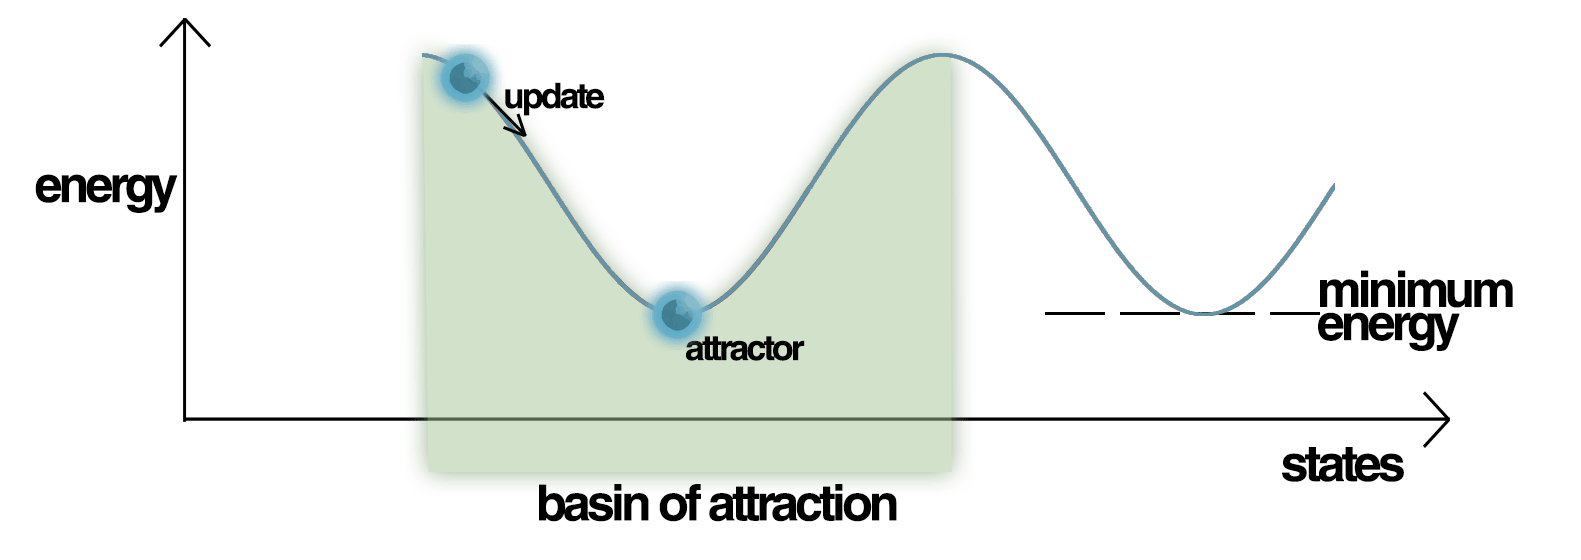
\includegraphics[scale=0.25]{energy_landscape.png}

\subsection{Stability and Capacity}

Concepts of stability and capacity are important in the analysis of Hopfield Networks. A neuron unit \( \epsilon_{i}^{\mu}\) is said to be stable if the update rule will not change its state. The mathematical condition for this is:

 \[x_{i} = sgn(\sum_{j=1}^{N}w_{ij}x_{j}) \]

Since we are using the Hebbian Rule, we can replace \(w_{ij}\) with
\(\sum_{\nu}\epsilon_{i}^{\nu}\epsilon_{j}^{\nu}\), resulting in:

\[ h_{i}^{\mu} = \frac{1}{N}\sum_{j} \sum_{\nu} \epsilon_{i}^{\nu}
						 \epsilon_{j}^{\nu}
						 \epsilon_{j}^{\mu}\]
 
 We will now isolate the contribution of neuron i, in order to get:
 
\[ h_{i}^{\mu} = \epsilon_{i}^{\nu} + \frac{1}{N}\sum_{j} \sum_{\nu\neq\mu} 			 					 \epsilon_{i}^{\nu}
						 \epsilon_{j}^{\nu}
						 \epsilon_{j}^{\mu}\]
 
 Now, the input for node i is made of two components: the first component depends on the node i itself, while the second component, called the \textbf{crosstalk term}, is directly dependent upon the neighbours of the node. 
 
 If we multiply the crosstalk term by \(-\epsilon_{i}^{\nu}\),  we get a quantity that will help us study the capacity:
 
 \[ C_{i}^{\nu}= -\epsilon_{i}^{\nu} \frac{1}{N}\sum_{j} \sum_{\nu\neq\mu} 			 			\epsilon_{i}^{\nu}
		       		 \epsilon_{j}^{\nu}
				 \epsilon_{j}^{\mu}\]
 
 If \( C_{i}^{\nu} \) is negative, then the cross-talk term has the same sign as unit i, and thus this value will not change \cite{lectureslides}. However, if \( C_{i}^{\nu} \) is positive and greater than 1, then \( \epsilon_{i}^{\nu}\) will change, so node i will become unstable. We will estimate the probability of \( C_{i}^{\nu} > 1 \)
 
 \textbf{UNFINISHED}
 
\subsection{Training using the Pseudo-Inverse Rule}

The pseudo-inverse rule makes use of the inverse of a matrix in order to perform the learning process. In contrast to the Hebbian Learning, it offers a higher capacity and performs better with correlated, linearly independent patterns. The weight matrix is computed as:

\[ w_{ij} = \frac{1}{N} \sum_{\mu\nu}\epsilon_{i}^\mu Q^{-1} \epsilon_{j}^\mu \]

In this case, Q is the overlap matrix:
\(  Q_{\mu\nu} = \frac{1}{N}\sum_{i}\epsilon_{i}^\mu \epsilon_{i}^\nu \)

%Locality and Incrementality
%I thought it would be best to be inserted here, since the reader has just been introduced to the second training rule, and can easily compare and reason out why these properties are useful
Now that we have introduced a second learning rule, it is worth mentioning a few desirable properties that neural network learning rules should aim to have. In Artificial Neural Networks, learning rules can be:
\begin{itemize}
 \item Local: each weight is updated using information available to neurons on either side of the connection.
 \item Incremental: new patterns can be learned without using information from the older patterns. When a new pattern is used for training, the new values for the weights only depend on the old values and on the bits of the pattern.
\end{itemize}

These properties are desirable, since learning becomes more biologically plausible. For example, since our brain is always learning new concepts, we can reason that learning is incremental. A learning system that would not be incremental would generally be trained only once, with a huge batch of training data.

It is important to mention that Hebbian Learning is both local and incremental, whereas the Pseudo-inverse learning rule is neither local nor incremental, since it depends upon the computation of an inverse matrix that contains information about all the patterns together.

\subsection{Training using the Storkey Rule}

The weight matrix of an attractor neural network is said to follow the Storkey learning rule if it obeys:

\[ w_{ij}^{\nu-1} = w_{ij}^{\nu-1}+
		    +\frac{1}{n}\epsilon_{i}^{\nu} \epsilon_{j}^{\nu} 
		    -\frac{1}{n}\epsilon_{i}^{\nu} h_{ji}^{\nu}
		    -\frac{1}{n}h_{ij}^{\nu} \epsilon_{i}^{\nu}
		    \]

where \( h_{ji}^{\nu} = \sum_{k=1,k\neq,j}^{n} w_{ik}^{\mu-1}\epsilon_{k}^{\mu} \) is a form of \emph{local field} \cite{storkey1997increasing} at neuron i.\\ 
		    
This rule is local, since the synapses take into account only neurons at their sides. This rule is slightly more powerful than the generalised Hebb rule, since it makes use of more information. Because of the action field, each neuron uses information from all the neighbours. As Storkey has showed in 1997, the capacity of the network trained with this rule is greater than compared to Hebbian rule \cite{storkey1997increasing}.






% Chapter 2 - part 2

%%%%%%%%%% Start TeXmacs macros
\newcommand{\nocomma}{}
\newcommand{\noplus}{}
\newcommand{\tmop}[1]{\ensuremath{\operatorname{#1}}}
\newcommand{\tmtextbf}[1]{{\bfseries{#1}}}
\newcommand{\tmtextit}[1]{{#1}}
\newcommand{\tmtexttt}[1]{{\ttfamily{#1}}}
\newenvironment{descriptioncompact}{\begin{description} }{\end{description}}
%%%%%%%%%% End TeXmacs macros


\section{Restricted Boltzmann Machines}

Hopfield networks are deterministic: training a network with the same patterns
will yield the same weights, and matching a pattern against the network will
always give the same result. This has the advantage of simplicity and ease of
testing. However, as mentioned before, there are spurious attractors in the
Hopfields network (linear combination of an odd number of training patterns).
Using stochastic updating rules will decrease the probability of being 'stuck'
in such a state. This resembles simulated annealing, but ensuring we are not
caught in a local minima (in the energy landscape).

Restricted Boltzmann Machines have been used for various purposes in recent
years
\cite{louradour2011classification} \cite{teh2001rate} \cite{nair2010rectified}
, most of it
conducted by Geoffrey E. Hinton at university of Toronto, Canada. They have a
simple structure: one layer of visible units and one layer of hidden units,
which form a bipartite graph, as in Figure. The patterns used to train the
network correspond to the visible (exposed units), while the hidden units
correspond to the attributes of the features we would like to learn. It is
worth mentioning that in the most common and simple form, both the visible and
hidden units take binary values. This is the approach we also adopted for our
implementation.

\ \ \ \ \ \ \ \ \ \ \ \ \ \ \ \ \ \ \ \ \ \ \ \ \ \ \ \ \begin{figure}[h]
  \centering
  \resizebox{300px}{300px}{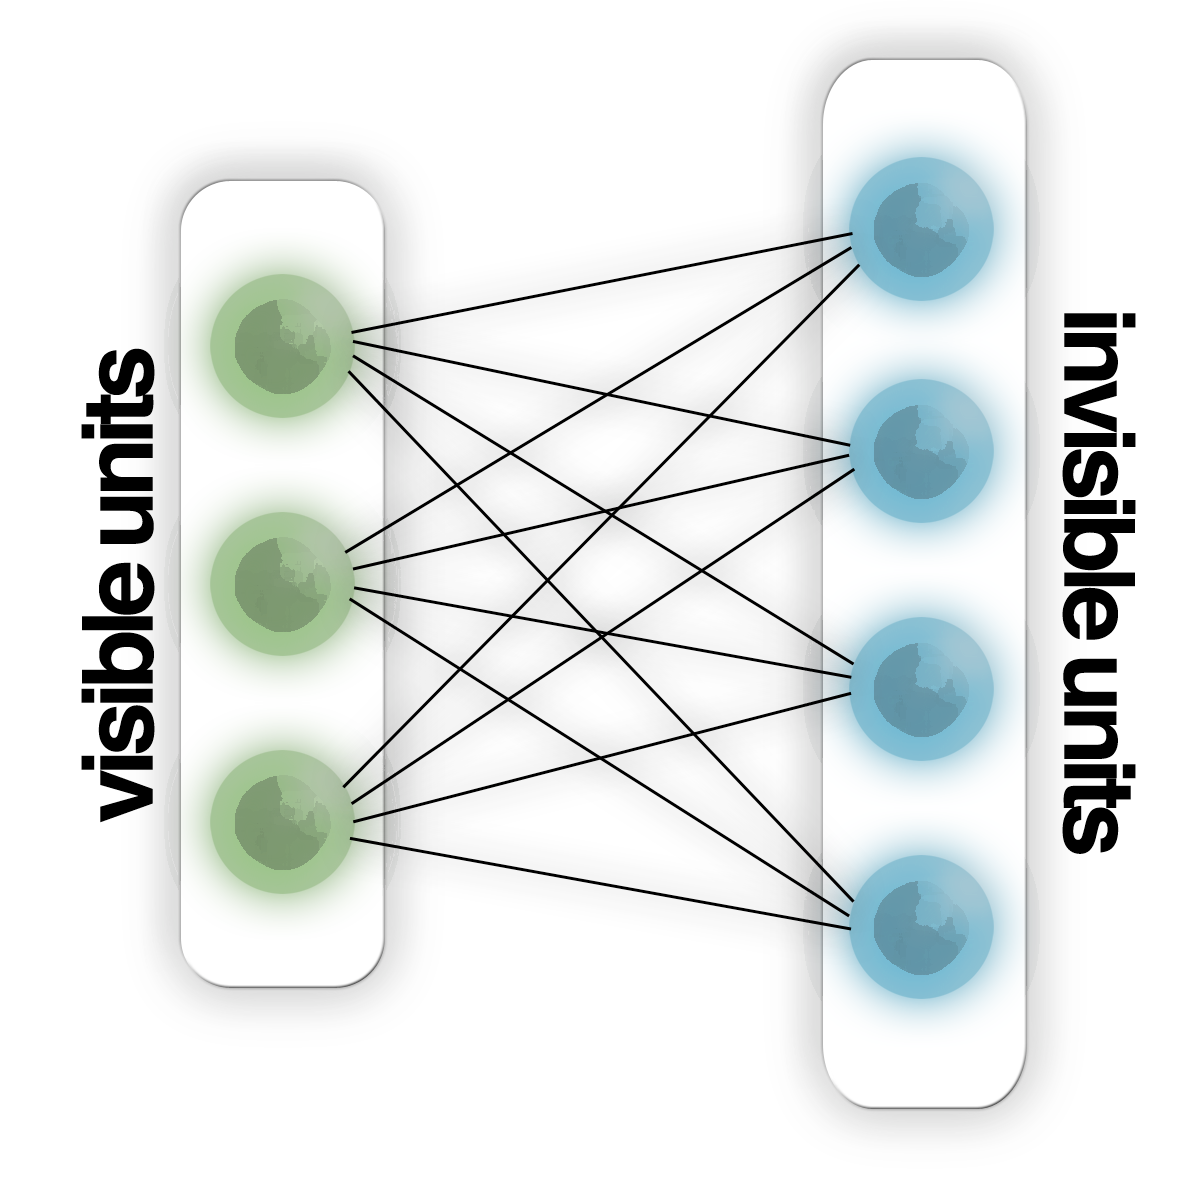
\includegraphics{RBM-1.eps}}
  \caption{Restricted Boltzmann Machine}
\end{figure}


The connections between the neurons in the two layers is symmetrical, so it
can be represented as a weight matrix which keeps the connection between hidden
and visible layers. A state of a Restricted Boltzmann machine is given by the
values of both the visible and given state. The corresponding Hopfield energy
formula for a state is given by :
\[ E (v, h) = - \sum_{i \in V} a_i v_i - \sum_{j \in H} b_j h_i - \sum_{i \in
   V, \nocomma j \in H \nocomma} v_i h_j w_{\tmtextit{\tmtextit{\tmop{ij}}}}
\]


where, $w_{\tmtextit{\tmtextit{}}}$is the weight matrix, $a$ and $b$are the
vectors of biases corresponding to the visible, respectively hidden layers. As
expected, $v$is vector of visible units and \tmtextit{h} is the vector of
hidden units.

We denote by \tmtextit{V} = \{1, .. \tmtextit{length} \tmtextit{v}\} , the
indices of a visible vector and by \tmtextit{H} = \{1, .. \tmtextit{length}
\tmtextit{h}\} the indices of a hidden vector.



\subsection{Probability of a state}

After traning, the network assigns a probability to each possible state, as
follows:
\[ p \left( v, h \right) = \frac{1}{Z} e^{- E \left( v, h \right)} \]
where Z is used to normalize the probabilities
\[ Z = \sum_{v, h} e^{- E \left( v, h \right)} \]
Thus, the probability the network asessings for a visibile vector \tmtextit{v}:
\begin{equation}
  p \left( v \right) = \sum_h \frac{1}{Z} e^{- E \left( v, h \right)}
\end{equation}

\subsection{Training the network}

The network can be trained such that one maximizes the probability of a training
pattern. The derivative of the log probability of a training vector (given by
(1)), is simple, as follows:
\[ \frac{\delta \log p \left( v \right)}{\delta w_{\tmop{ij}}} = < v_i h_i
   >_{\tmop{data}} - < v_i h_i >_{\tmop{model}} \]
Due to the fact that the Restricted Boltzmann Machine can be represented as a bipartite graph, it is easy
to attain an \tmtextit{unabiased} sample of the hidden units, given the
visible units.
\begin{equation}
  p \left( h_j = 1 \left|  \right. v \right) = \sigma \left( b_j + \sum_{i \in
  V} v_i w_{\tmop{ij}} \right)
\end{equation}
For the visible units, the same formula gives a \tmtextit{biased} sample of
the visible units.
\begin{equation}
  p \left( v_i = 1 \left|  \right. h \right) = \sigma \left( a_i + \sum_{j \in
  H} h_j w_{\tmop{ij}} \right)
\end{equation}


where $\sigma = \frac{1}{1 \noplus + e^{- x}}^{}$, is the logistic sigmoid
function.

There are ways of getting an unbiased sample of the visible units, but they
are very time consuming. In practice, the contrastive divergence algorithm is
used as a faster substitute. The visible units are set to a training vector
and the binary states of the hidden vector are computed using (2). These
binary units are used to \tmtextit{reconstruct} the states of the visible
vector using (3).

The training rule then becomes:
\[ \Delta w_{\tmop{ij}} = \lambda \left( < v_i h_i >_{\tmop{data}} - < v_i h_i
   >_{\tmop{reconstruction}} \right) \]
We note that the above training rule has the desired properties for modeling
the biological brain: it is both \tmtextit{local} and \tmtextit{incremental}.
Angle brackets \ denote the expected value under the given distribution by the
following subscript.



\subsection{Using Restricted Boltzmann Machines for classification}

As suggested by Hinton in section 16 \cite{hinton2010practical}, there are various ways of using Restricted
Boltzmann Machines for classification. We have employed two methods, one which
we developed ourselves and another one described in the paper. The latter is adding
another set of visible units, called the \emph{classification units}.



\ \ \ \ \ \ \ \ \ \ \ \ \ \ \ \ \ \ \ \ \ \ \ \begin{figure}[h]
  \ \ \ \ \ \ \ \ \ \ \centering
  \resizebox{350px}{350px}{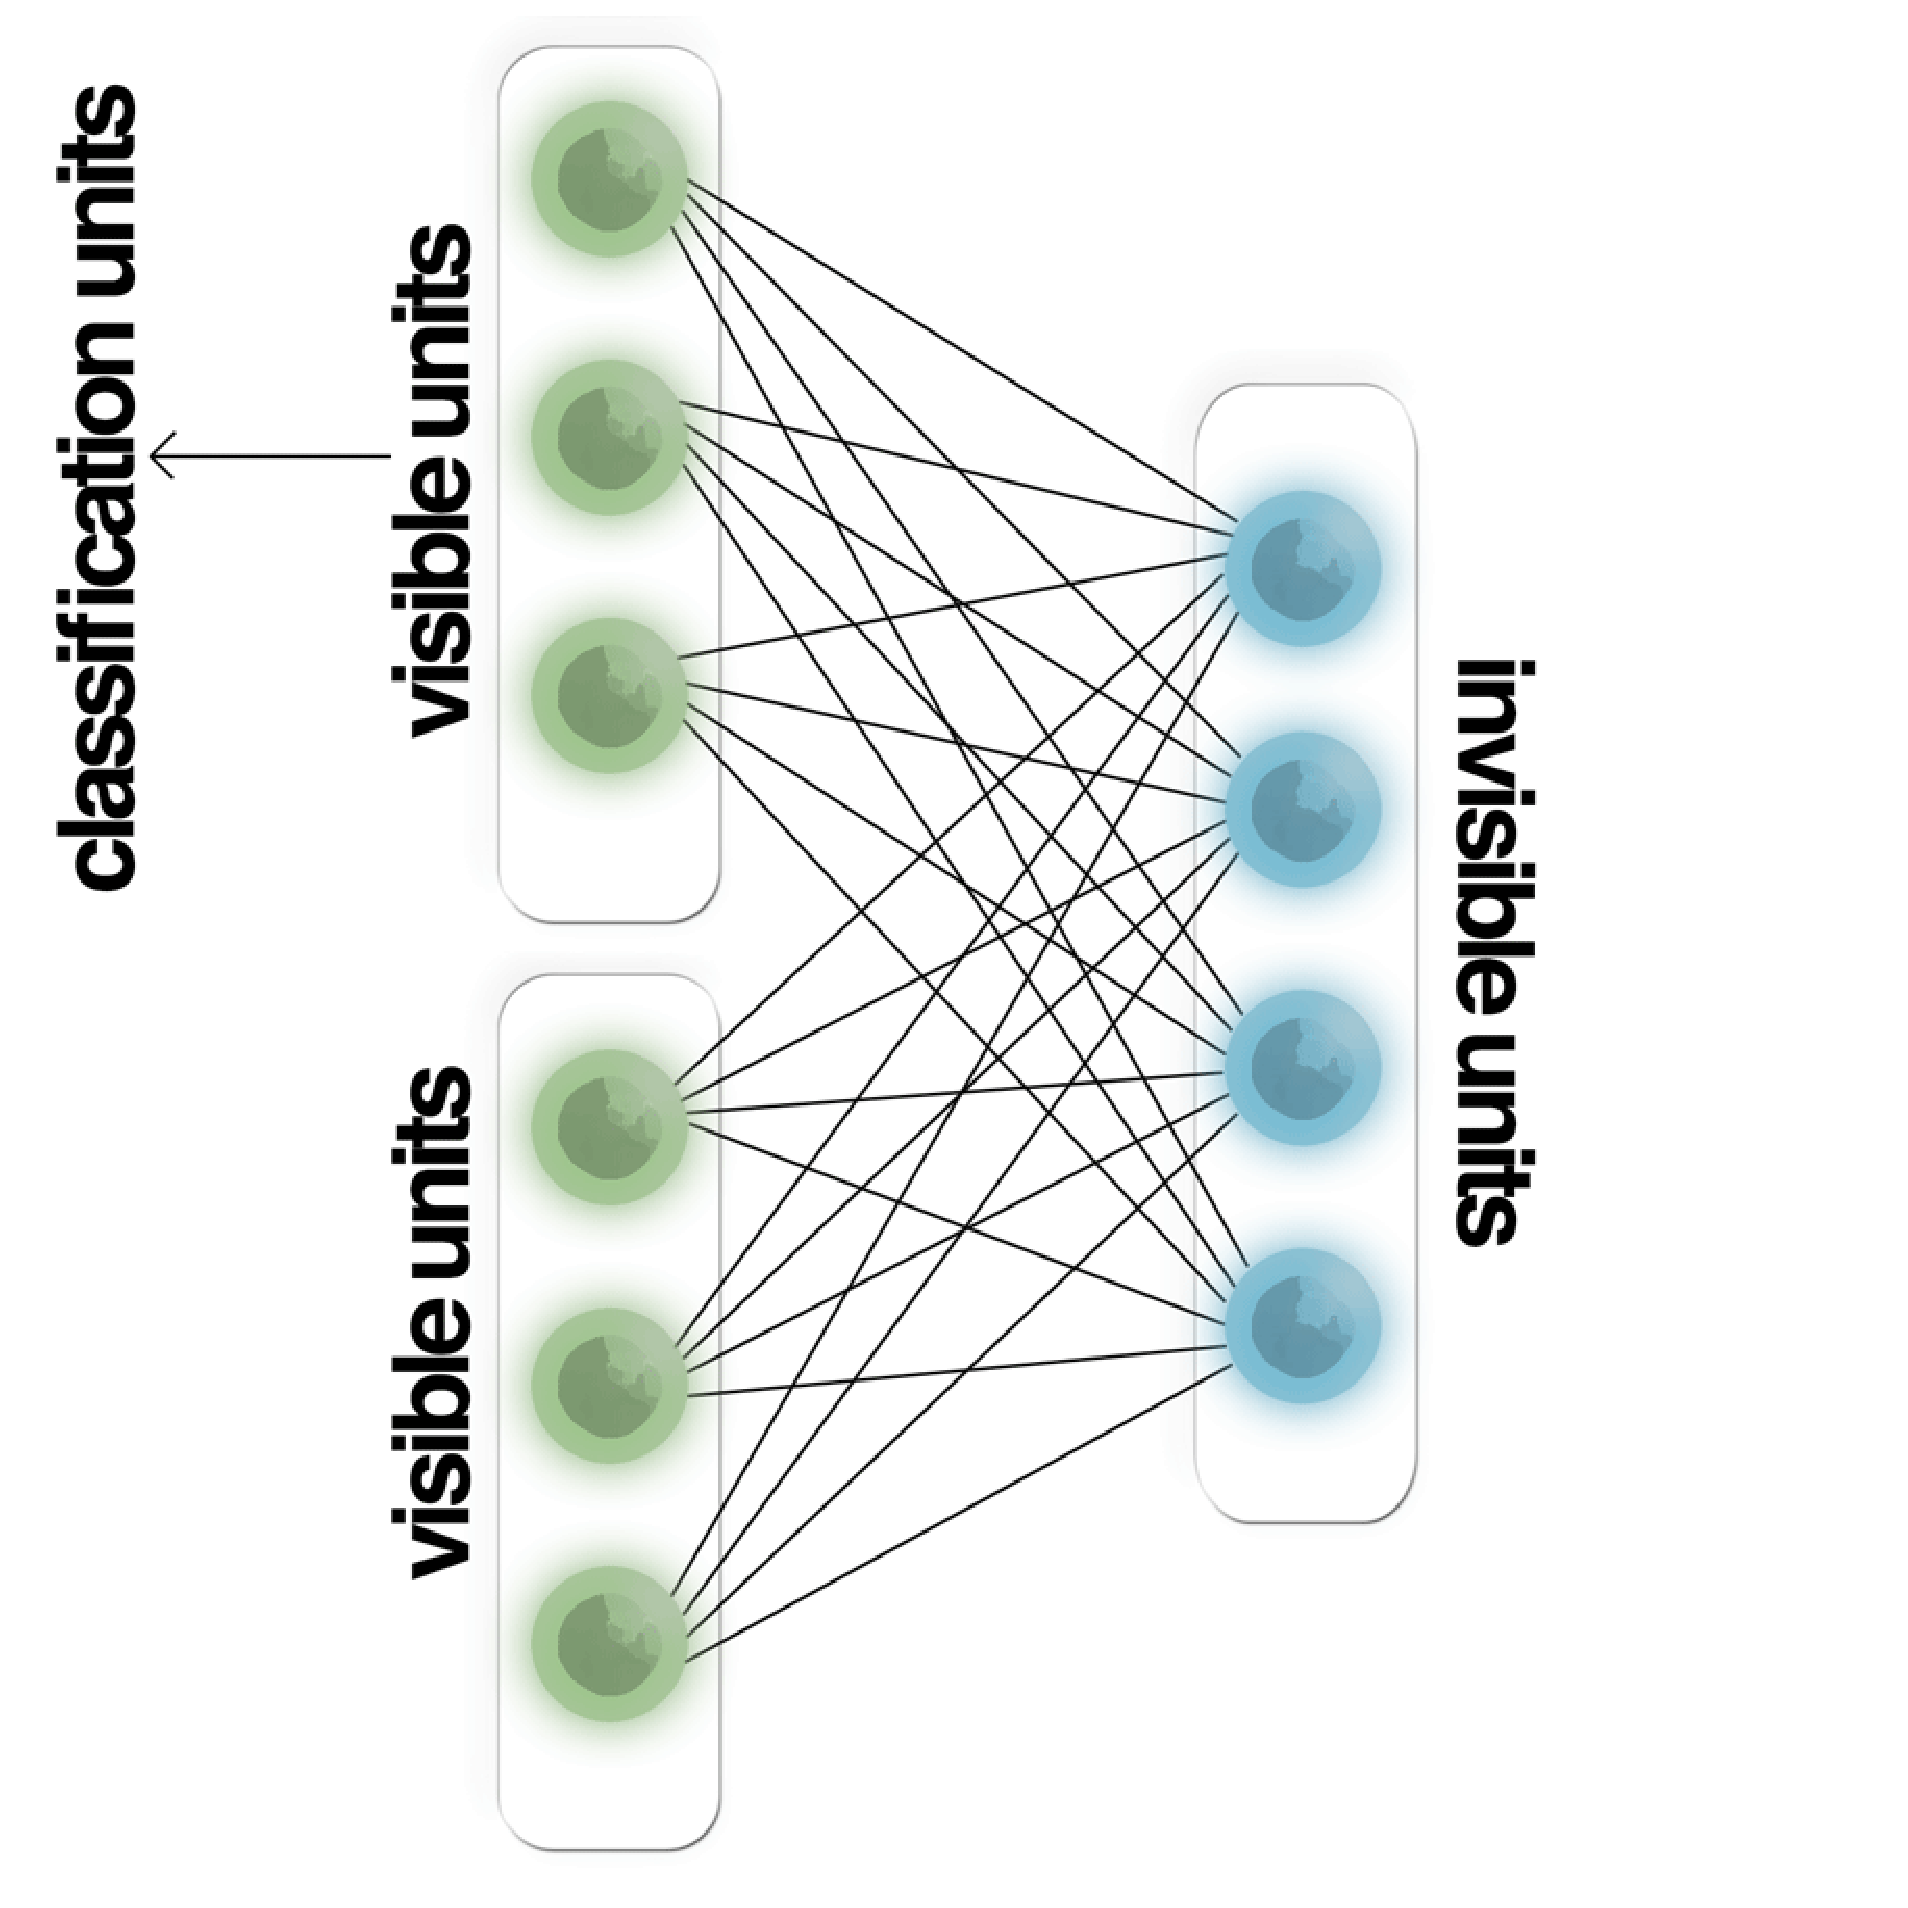
\includegraphics{RBM-2.eps}}
  \caption{Classification Boltzmann machine}
\end{figure}



The vector of hidden units is used to model the joint distribution between a
vector of inputs v and a target (classification) vector y. The classification
vector y corresponds to a class. It's length is given by the number of
classes. $y = e_c$, where c is the class the vector is modeling ($e_c$ is a
vector with all zeros, expect from the position c, where it is 1).

As seen from Figure 2, one now needs to weight matrices, which we will denote
by \tmtextit{W}(the weight matrix between the visible units and hidden ones) \
and U (the weight matrix and between the classification units and hidden
ones). Vectors \tmtextit{b}, \tmtextit{c}, \tmtextit{d} correspond to the
vector of biases for the visible units (training patterns), hidden units and
classification units, respectively.

The energy function for this model is:
\[ E \left( v \nocomma, y, h \right) = - d^T y - c^T h - b^T v - h^T W v - h^T
   U y \]
Which gives rise to the following formula for the probability of a configuration
\tmtextit{v}, \tmtextit{y}.
\[ p \left( v, y, h \right) = \frac{e^{- E \left( v \nocomma, y, h
   \right)}}{Z} \]
where \tmtextit{Z} is the normalizing constant. Thus,
\[ p \left( v, y \right) = \sum_h p \left( v, y, h \right) = \sum_h \frac{e^{-
   E \left( v \nocomma, y, h \right)}}{Z} \]
The distribution used for the Classification Boltzmann Machine are the
following:
\begin{equation}
  p \left( h_i = 1 \left| v, y \right. \right) = \sigma \left( c_j + \noplus
  \noplus W_j v \noplus + U_j y \right)
\end{equation}
\begin{equation}
  p \left( v_i = 1 \left| h \right. \right) = \sigma \left( b_j + \noplus
  \noplus h^T W^i  \right)
\end{equation}
\begin{equation}
  p \left( y = e_c \left| h \right. \right) = \frac{e^{d^T e_c \noplus + h^T
  Ue_c}}{N}
\end{equation}
where N is the normalizing constant $\sum_c$ $e^{d^T e_c \noplus + h^T Ue_c}$.

Note that we denote by $W_i$ the row \tmtextit{i} of matrix \tmtextit{W}, and
by $W^i_{}$ the column \tmtextit{i} of matrix \tmtextit{W}.



Valuable reference for this was given to us from
\cite{louradour2011classification} and
\cite{larochelle2008classification}.

\subsection{Learning}

Contrastive divergence can be used to train the network, giving rise to the
following update rules:


\begin{eqnarray*}
  b'  & = & b + \lambda \left( v - v_{\tmop{sampled}} \right)\\
  c'  & = & c + \lambda \left( h_{\sigma} - h_{\sigma \tmop{sampled}}
  \right)\\
  d'  & = & d + \lambda \left( y - y_{\tmop{sampled}} \right)\\
  W'  & = & W + \lambda \left( h_{\sigma} v^T - h_{\sigma \tmop{sampled}}
  v_{\tmop{sampled}}^T \right)\\
  U' & = & U + \lambda \left( \left. h_{\sigma} y^T - h_{\sigma
  \tmop{sampled}} y_{\tmop{sampled}}^T \right) \right.
\end{eqnarray*}
where we denote by $x'$ the new value of parameter x. $v_{\tmop{sampled}} $and
$y_{\tmop{sampled}} $are obtained by sampling the distributions in (5) and
(6).
\begin{eqnarray*}
  h_{\sigma} & = & \sigma \left( c_j + \noplus \noplus W_j v \noplus + U_j y
  \right)\\
  h_{\sigma \tmop{sampled}} & = & \sigma \left( c_j + \noplus \noplus W_j
  v_{\tmop{sampled}} \noplus + U_j y_{\tmop{sampled}}  \right)
\end{eqnarray*}
\subsection{Classification}
\[ p \left( y = e_c \left| v \right. \right) = \frac{e^{- F \left( v \nocomma,
   e_c \right)}}{\sum_d e^{- F \left( v \nocomma, e_d \right)}} \]
where $F \left( v \nocomma, e_c \right) $is the \tmtextit{free energy
function}
\[ F \left( v \nocomma, e_c \right) = - d^T y - \sum^H_{j = 1}
   \tmtextit{\tmtextit{s}} \left( c_j + \noplus \noplus W_j v \noplus + U_j y
   \right) \nocomma \]
where $s \left( x \right) = \log \left( 1 + e^x \right) $



The implementation of the Classification Boltzmann Machine can be found in

\tmtexttt{ClassficationBoltzmannMachine.hs. }



\subsection{New method}

Another method we have employed using Boltzmann Machines was created by us. We
have never seen this approach used somewhere else. Instead of creating 2 types
of visible units, we use the simple Restricted Boltzmann Machine, with one
type of visible units (and hence a single matrix). For each training vector
we append the classification at the end. The classification is represented as
a binary vector, either as above, by using $e_c$, where c is the
classification of the current pattern, or even in a more compressed manner, by
creating the binary vector using the representation in base 2 of class c.

\ \ \ \ \ \ \ \ \ \ \ \ \ \ \ \ \ \ \ \ \ \ \ \ \ \ \ \ \ \ \ \ \ \ \ \ \ \
\ \ \

\ \ \ \ \ \ \ \ \ \ \ \ \ \ \ \ \ \ \ \ \ \ \ \ \ \ \ \ \ \ \ \ \ \ \ \ \

\ \ \ \ \ \ \ \ \ \ \ \ \ \ \ \ \ \begin{figure}[h]
  \ \ \ \ \ \ \ \ \ \ \ \ \
  \centering
  \resizebox{350px}{350px}{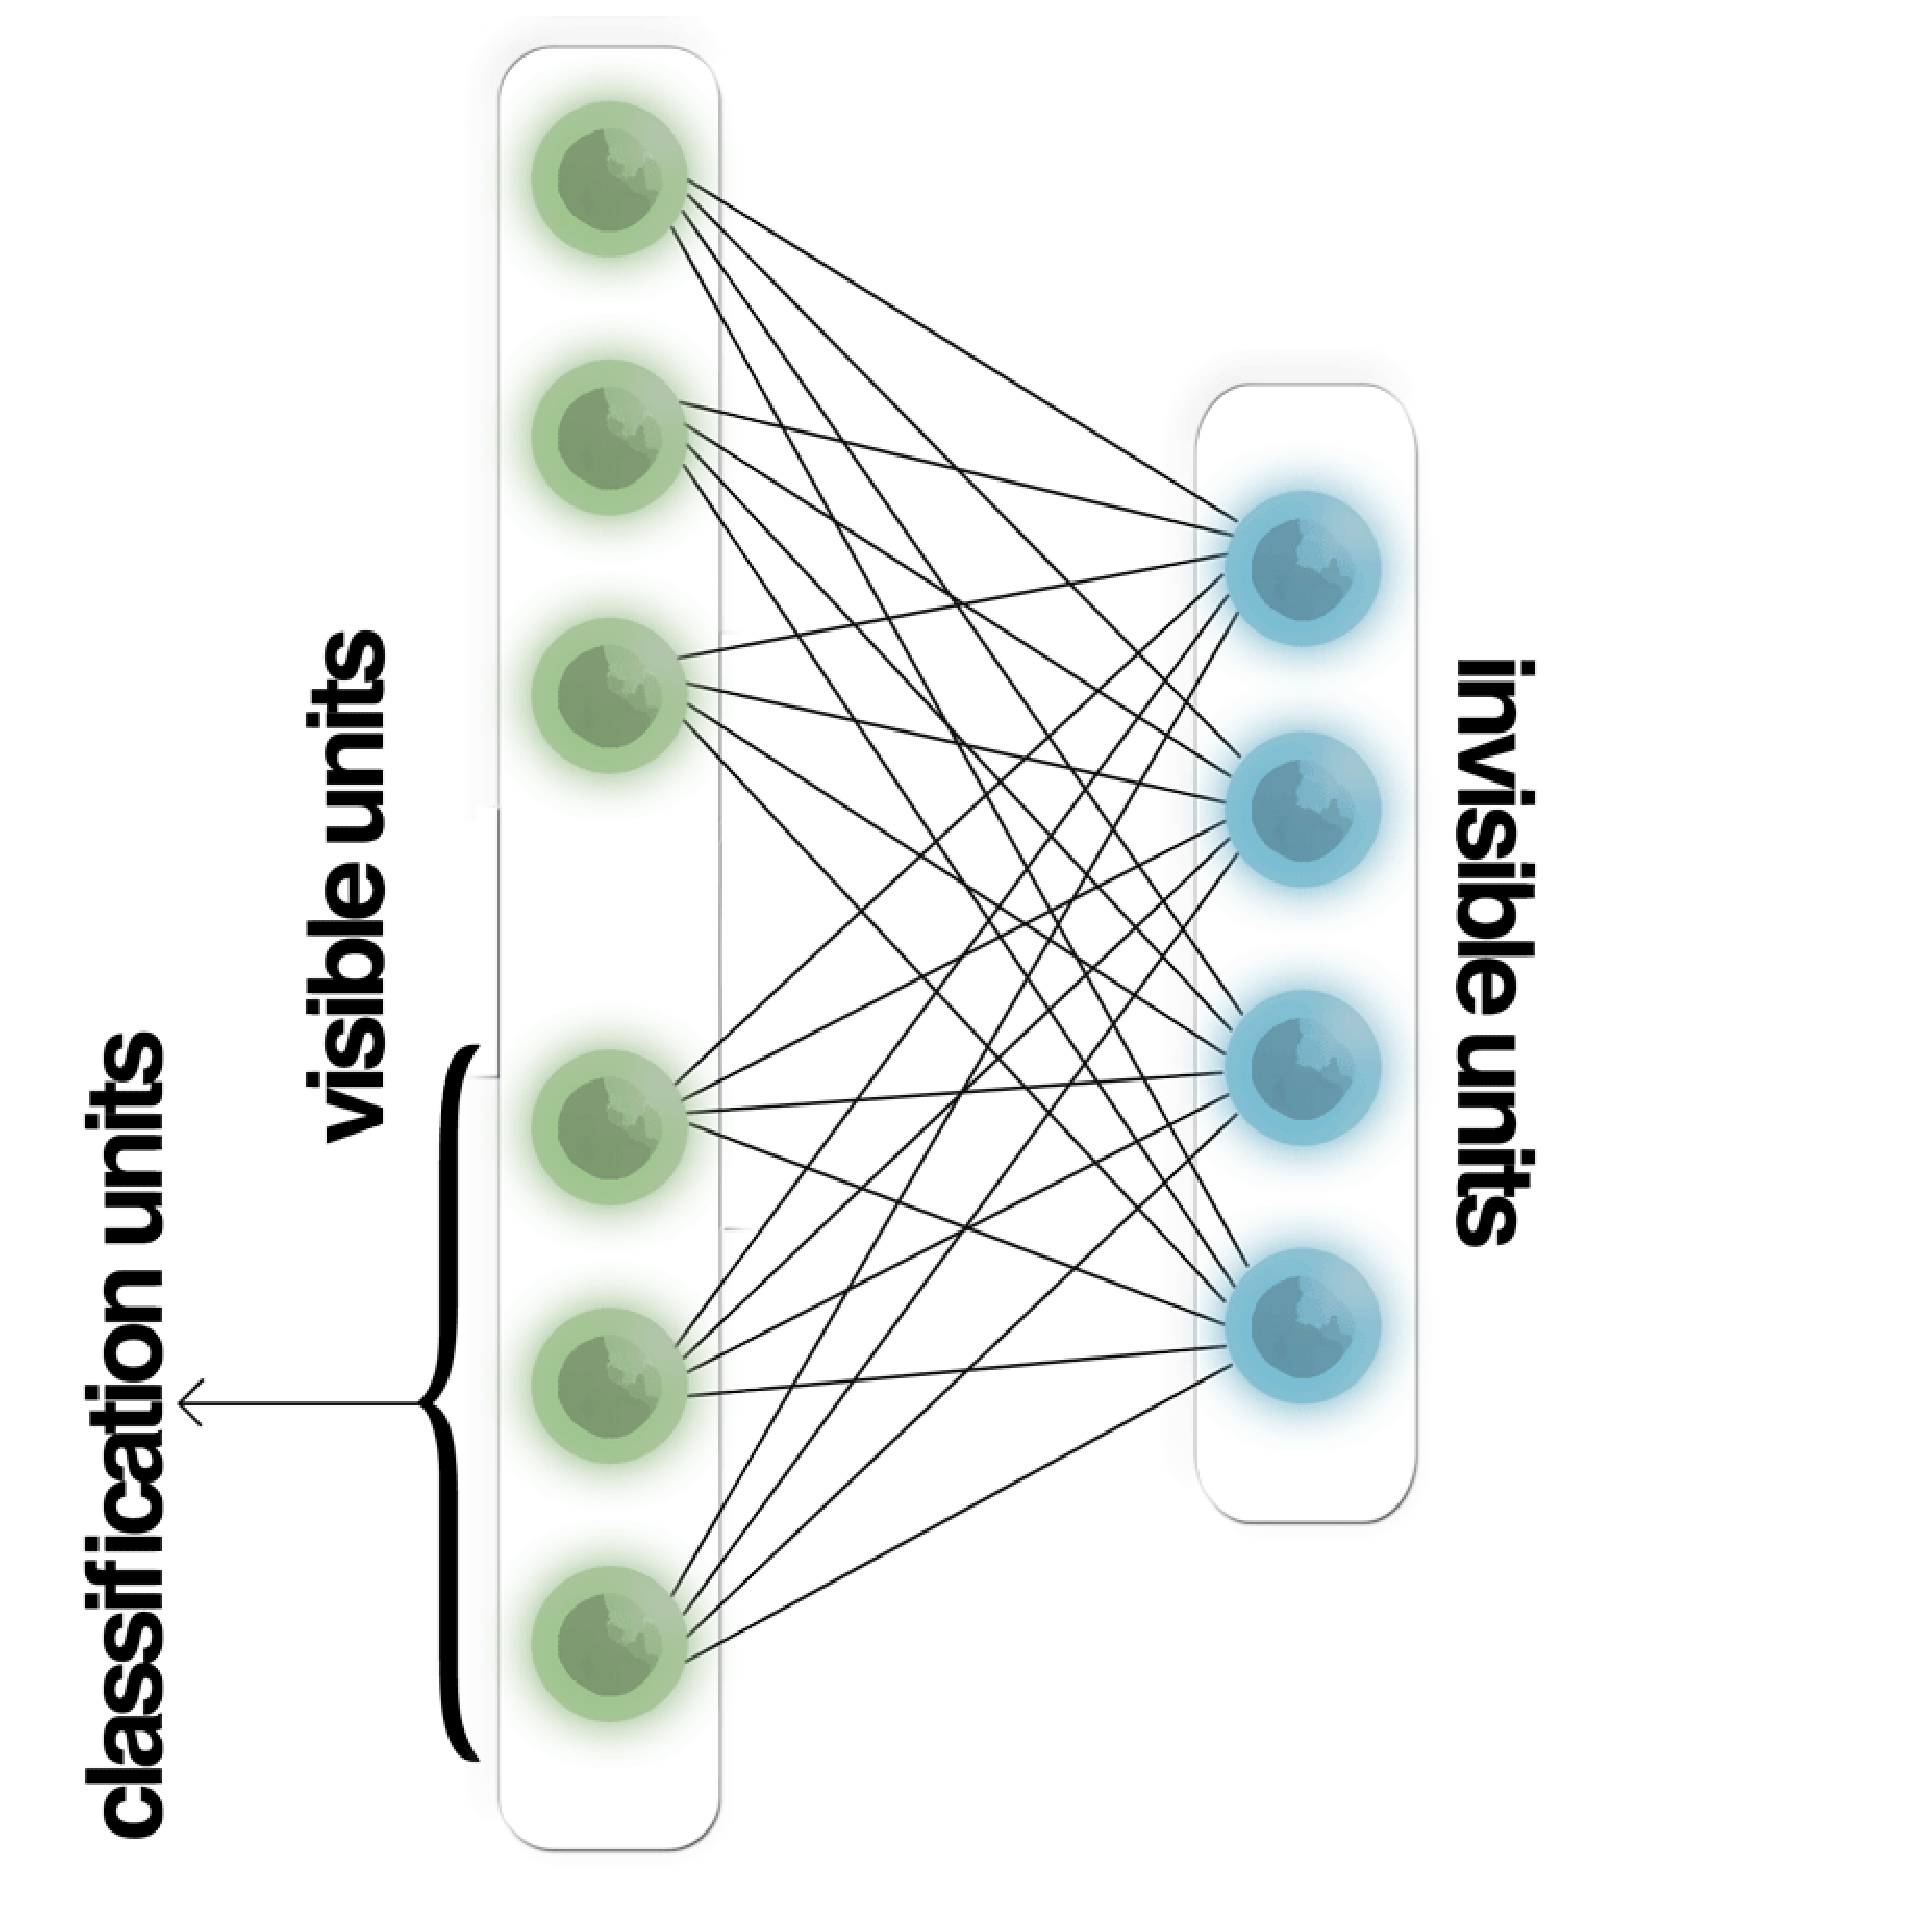
\includegraphics{RBM-3.eps}}
  \caption{Boltzmann machines according to our new method}
\end{figure} \ \ \ \ \ \ \ \ \ \ \ \ \ \ \ \ \ \ \ \ \ \ \ \ \ \ \ \ \ \ \ \ \
\ \ \ \ \ \

\ \ \ \ \ \ \ \ \ \ \ \ \ \ \ \ \ \ \ \ \ \ \ \ \ \ \ \ \ \ \ \ \ \

The training is done in the usual way, but with the complete vectors (actual
pattern and classification). In our case, as different patterns ought to have
different classifications, we use as class the index of the pattern in the list
(with removed duplicates) of training patterns.

When a pattern needs to be matched to one of the training patterns for
recognition, one uses the log probability (given using ...) to compute the
probability of each of the classifications, and choses the one with maximum
probability.



\begin{figure}[h]
  \centering
  \resizebox{622px}{182px}{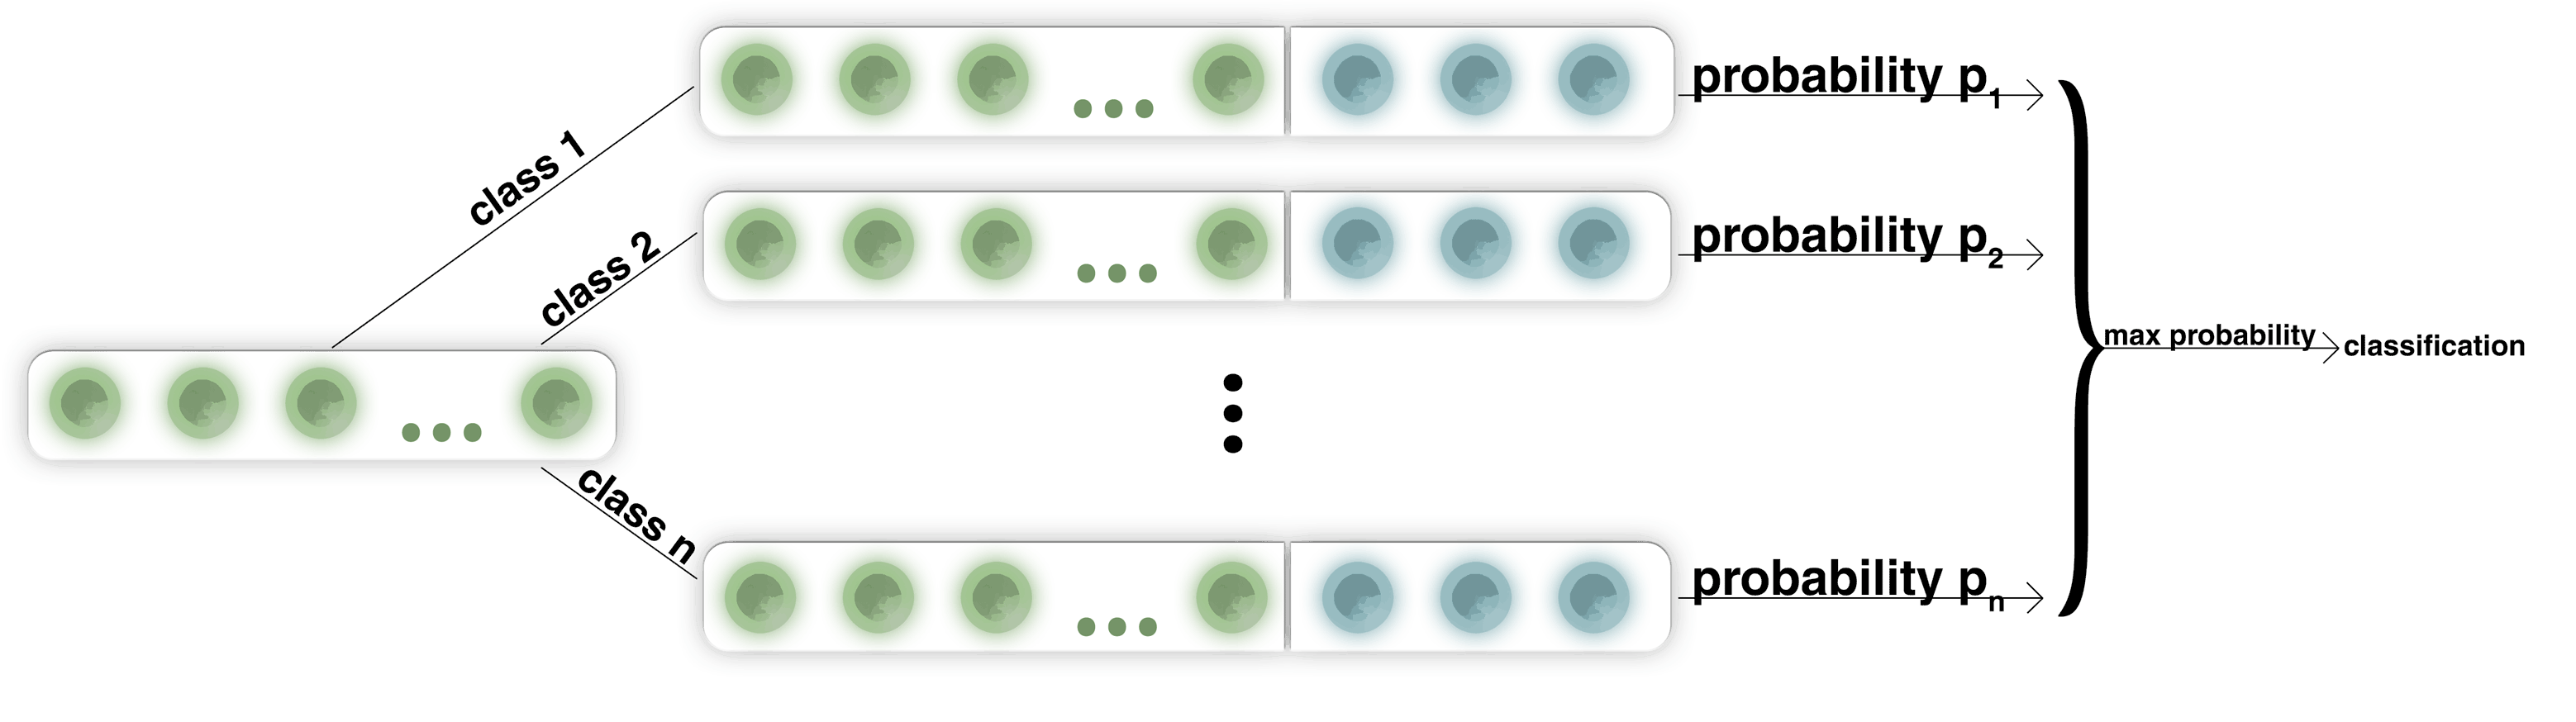
\includegraphics{RBM-4.eps}}
  \caption{The recognition process in the new Boltzmann machine.}
\end{figure}



As given in \cite{hinton2010practical}, the log
probability is  given by:
\[ \tmtextit{\log} \left( \tmop{class} = c \left| v \right. \right) =
   \frac{e^{- F_c \left( v \right)}}{\sum_{c'} e^{- F_{c'} \left( v
   \right)}} \]
\[ F \left( v \right) = - \sum_{i \in V} v_i a_i - \sum_{j \in H} \log \left(
   1 \noplus + e^{x_j} \right) \]


where $x_j = b_j + \sum_i w_{ij_{}} v_j$



The implementation of this procedure can be found in
\tmtexttt{RestrictedBoltzmannMachine.hs.}



% Chapter 3
\chapter{Exploring The Hopfield Model}
% This is where we describe our experiments. We insert plots, images, ....

We started out the analysis by experimenting with converge of patterns. We shall present two experiments, that provide some interesting insight for the reader into the Hopfield Model.

\section{Facial Recognition for Police criminal records}

This experiment describes how the Hopfield network might be used by a Police Office, in order to identify criminals. Since the police has a big database that contains facial images of criminals, the network can perform identify, given an image, which criminal is depicted.

Before being sent to the Hopfield model, the image suffers a few normalizing transformations:
\begin{enumerate}
 \item the background is completely removed
 \item the image is scaled to 25x25 pixels.
 \item conversion first to grayscale, and then to only black or white pixels takes place
\end{enumerate}

In figure \ref{fig:criminal}, we present the convergence series for the input image of a criminal. The network used for this experiment had 400 neurons, running on images of 20x20 pixels. It clearly illustrates the how efficient the networks can be in these scenarios. However, the network might also convert to to spurious patterns, which might create problems in certain situations. See section \ref{spurious_patterns} for a more detailed description.

\begin{figure}[h]
  \centering
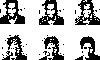
\includegraphics[scale=2]{images/convergence/all.png}
\caption{Convergence sequence for a criminal in the police database}
\label{fig:criminal}
\end{figure}

Furthermore, we have developed a GUI, powered by the underlying recognition core, to provide a friendly user experience, in addition to providing interactive facilities (figure \ref{fig:gui}). An overview of our the recognition system can be found in figure ~\ref{fig:system}.

\begin{figure}[h]
  \centering
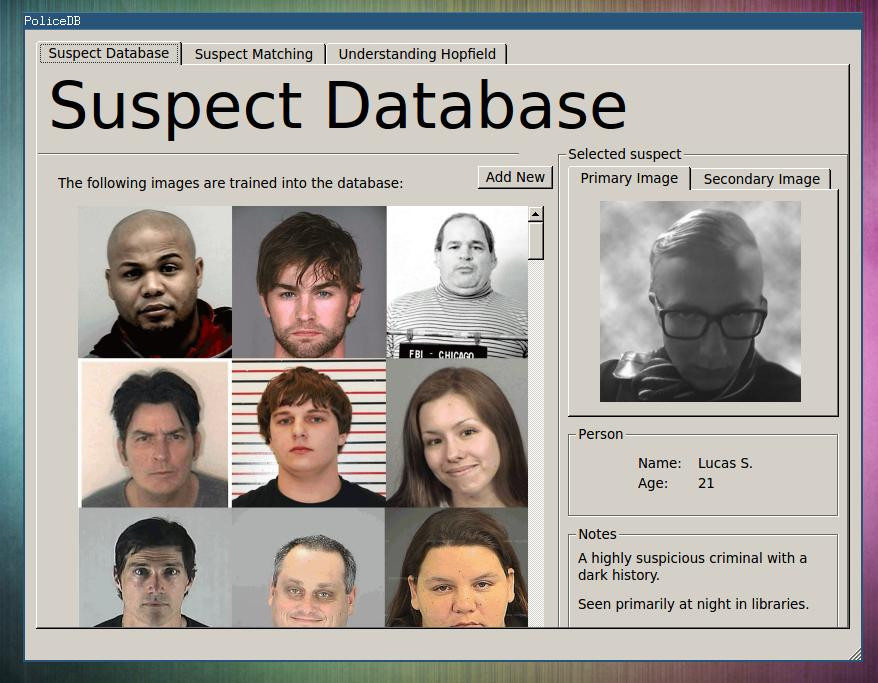
\includegraphics[scale=0.3]{screenshots-small/gui1.jpg}
\caption{GUI for a criminal record recognition system.}
\label{fig:gui}
\end{figure}

\begin{figure}[h]
  \centering
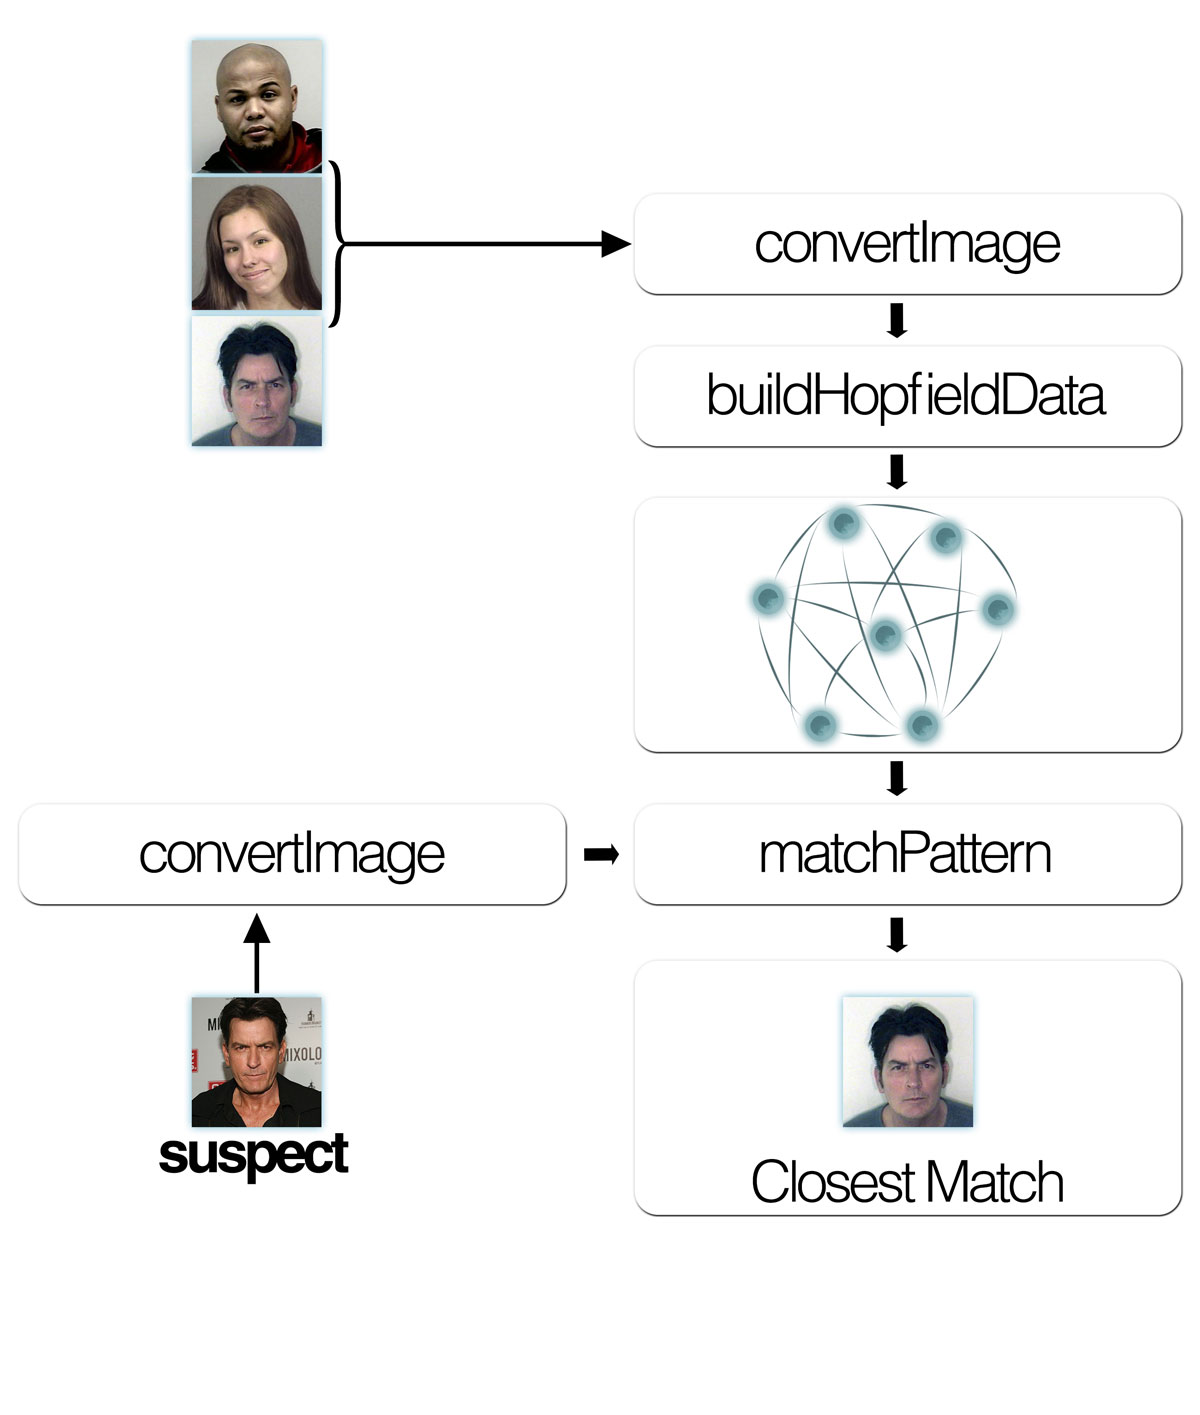
\includegraphics[scale=0.3]{recognition.jpg}
\caption{Outline of the Recognition System demonstrating how the various system components interact}
\label{fig:system}
\end{figure}


\section{Further analysis}

Our initial aim was to explore various properties of the attractors in a Hopfield Network. We are interested in studying, testing or challenging several ideas about the neural network:
\begin{itemize}
 \item Clusters of attractors: We are interested to see how the Hopfield network behaves when learning similarly correlated patterns. This implies training the network with a cluster of attractors, which will lower the capacity of the network. We believe that basin sizes will get smaller as the patterns get closer to each other.
 \item Super-Attractors: Find out what happens if the network is trained several times with the same pattern. We believe this super-attractor will have a larger basin size compared to the other attractors.
 \item Convergence: We plan to train the network with different types of attractors and find out to which ones patterns tend to converge.
\end{itemize}

\section{Basins of Attraction}
%I think we should move the measurements for the basins of attraction in here.
A basin of attraction for a particular attractor \(\alpha\) is defined as the set of all states that will eventually converge to \(\alpha\), under repeated update. Here, we are particularly interested in finding a way to measure the size of such a basin of attraction. A large basin size would provide stability for the attractor, since the states in the neighbourhood would converge to it. A small basin size for an attractor would mean that the network might never recall the pattern corresponding to that attractor.

\subsection{Measuring the Basin Size using the Storkey-Valabregue technique}
\label{storkey_basin_size}

 A large part of our experiments were thus dedicated to measuring basin sizes of different attractors, clusters of attractors and a newly introduced concept of \emph{Super-Attractors}, in section ~\ref{super_attractors}.

 A recognised scientific method for calculating the basin size is the Storkey-Valabregue measurement. This can be computed as follows:

 \begin{enumerate}
  \item Initially n = 1
  \item Choose an initial fixed point corresponding to a stored pattern \(\mu\)
  \item \label{itm:choose radius} Choose some initial normalised Hamming radius \(r=r_{0}\)
  \item Let the set A be all the states Hamming-distant \( nr \) from the fixed point
  \item Sample 100 states from A
  \item Calculate how many of these states are attracted to the fixed point. Denote this number \( t_{\mu}(r) \)
  \item If \( t_{\mu}(r) \) is smaller than 90, stop and return \(nr\)
  \item Increment \(n\) by a suitable amount and repeat from (\ref{itm:choose radius})
  \item Repeat for each attractor.
 \end{enumerate}

% TODO: This algorithm is implemented in the Haskell function ...


\section{Generating Clusters of Attractors}

There are various ways of generating clusters of attractors (i.e. attractors that have a low Hamming distance between each other). We shall present two different methodologies that can be used to generate them.

One way is to start with a root pattern and then reverse each bit with a probability p. The new patterns can be interpreted as noisy versions of the root pattern. We shall denote this procedure T1.

\subsection{Generating Gaussian-Distributed Clusters}

Another objective of this work was to analyse patterns that are extracted according to a Gaussian distribution with a specific mean and variance.

Since the state space is \( 2^N \) for a network of N neurons, the Gaussian Distribution will have to be defined over a huge set of states. This is highly non-trivial, since we are dealing with binary patterns, that cannot be ordered in an easy way.

In this case, we will use Federico's method for sampling Gaussian distributed patterns \cite[p.~33]{federico}. We tackle this issue using the simplest possible approach: to draw numbers from a Normal Distribution and then translate them into patterns that will preserve the distance between them. Formally, if \(x\) and \(y\) were drawn and \( |x-y|=\delta\), then the Hamming distance between the encoded patterns \(x'\) and \(y'\) would also be \( d(x',y')=\delta\).

\subsubsection{Encoding of the patterns}

In order to encode a number into a binary pattern, we first round the number to the nearest integer. Let k be the integer obtained as such. Now, from left to right, we set to 1 all the bits in locations 1..k of our pattern. The remaining bits are set to -1.

For example, if the pattern size is 7 and the integer obtained is 4, we get the following pattern: [1,1,1,1,-1,-1,-1].

\subsubsection{Limitations of the encoding}

Although the method has a big advantage for simplicity, we can only obtain N different patterns out of all \( 2^N\) patterns available in the state space. However, we can regain capacity if we start flipping bits, while at the same time keeping constant the hamming distance to some certain mean pattern \(\mu\).

Another idea would be to extend our distribution to a multi-variate distribution. In this case, the capacity of the network would increase from \(N\) to \(\frac{n}{k}^k\), where k is the number of dimensions.

Unfortunately, we did not have enough time to implement these ideas, so we only experimented with the naive encoding of patterns described above.


\section{First experiments with basin sizes}
\label{sec:fexp}

In this section we shall introduce the experiments that we used to analyse various properties of the Hopfield Network. We remind the reader about the two methods that we are going to use for generating clusters of attractors:
\begin{itemize}
 \item T1: We start with a root pattern \(\mu\), and generate patterns by flipping each bit from \(\mu\) with probability \(p\).
 \item T2: This method is generating Gaussian-distributed patterns. We sample several numbers from a normal distribution with a certain mean and variance, and then encode each number into patterns of the form [1,1,1,-1,-1].
\end{itemize}


\subsection{Basin Size for One Cluster using T1}

Our first experiment is showing us the basin sizes for increasing values of p, the probability of flipping a bit. Method T1 is used, for a Hopfield Network of N neurons.

\begin{easylist}[enumerate]
\ListProperties(Style2*=,Numbers=a,Numbers1=R,FinalMark=.)
& We generate a random pattern \(\mu\)

& For all values of probability p from 0 to 0.5

    && Starting from \(\mu\) we generate P patterns using T1, and give them to the Hopfield network in order to be learned according to Hebb or Storkey rule.

    && We measure the basin size for all the patterns learned using the Storkey-Valabregue measurement and take their mean.
\end{easylist}

\begin{figure}[h]
  \centering
  \begin{tikzpicture}
\begin{axis}[
xmin = 0,
ymin = 0,
xlabel = $p$-value,
ylabel = Average Basin Size
]

\addplot [
color = black,
mark = *, % A filled circle
only marks,
smooth  % draw smooth curve
] table [
y = mean
] {data-T1-onecluster-100.csv};

\end{axis}
\end{tikzpicture}

\caption{Average Basin size of patterns belonging to one cluster generated using T1}
\label{fig:plot-T1-onecluster}
\end{figure}

\subsubsection{Comments}

The results are displayed in figure \ref{fig:plot-T1-onecluster}. This initial experiment is confirming not only what Federico obtained \cite{federico}, but also what we already know from theory: A Hopfield network that is trained with similar patterns loses capacity. Although we are not measuring capacity here, the basin size is strongly correlated to that.

Initially, when p is zero, we observe a huge value of 24 for the basin size. This is easily explained, since all the patterns generated are the the same as the root pattern. Subsequently, the network is trained with the same patterns that have the effect of creating a super-attractor with a huge basin size.

When p is between 0 and a critical value of 0.35, the basin size is 0, since the patterns are too close to each other and don't have enough space to fit basins of attraction between them. As soon as p goes over 0.35, the basins start to increase until a maximum size of 11.


\subsection{Basin Size for Two Clusters using T1}

This experiment is similar to the previous one, however it contains two clusters this time. The value \(p_{1}\) for one cluster will stay the same (fixed at 0.45), while \( p_{2}\), corresponding to the second cluster, will vary in the range [0-0.5]. Method T1 is used, for a Hopfield Network of N neurons. The procedure is given below:
\newline
\begin{easylist}[enumerate]
\ListProperties(Style2*=,Numbers=a,Numbers1=R,FinalMark=.)
& We generate 2 random patterns \(\mu_{1}\) and \(\mu_{2}\), corresponding to clusters \( C_{1} \) and \( C_{2} \).

& We generate P patterns for \( C_{1} \), using T1 with associated probability \( p_{1}=0.45\).

& For all values of probability \( p_{2} \) from 0 to 0.5

    && Starting from \(\mu_{2}\) we generate P patterns using T1 with associated probability \( p_{2} \), and give them to the Hopfield network in order to be learned according to Hebb or Storkey rule.

    && For both sets of patterns, we measure the mean basin size using the Storkey-Valabregue measurement and plot the values on the graph.
\end{easylist}

We will be interested to observe how can the probability p influences the basin sizes. For this reason, we have run two experiments, in which we are outputting the basin sizes for cluster 1, in which p varies. The

\subsubsection{Comments}

\begin{figure}[h]
  \centering
  \begin{tikzpicture}
\begin{axis}[
xmin = 0,
xmax = 0.5,
ymin = 0,
xlabel = p-value of cluster 2,
ylabel = Average Basin Size,
width=12cm,
height=9cm
% legend
% legend style={at={(1,0.5)},anchor=east}
]

\addlegendentry{Cluster 1 with $p$ = 0.2} ;

\addplot [
color = red,
mark = x, % A filled circle
% mark = none,
only marks,
smooth  % draw smooth curve
] table [
y = mean-new
] {data-T1-twocluster-100-0.4.csv};

\addlegendentry{Cluster 1 with $p$ = 0.4} ;


\addplot [
color = blue,
mark = triangle, % A filled circle
only marks,
smooth  % draw smooth curve
] table [
y = mean-new
] {data-T1-twocluster-100-0.2.csv};

\addlegendentry{Cluster 1 with $p$ = 0.2} ;



\end{axis}
\end{tikzpicture}

\caption{Average Basin size of patterns belonging to Cluster 2, generated using T1}
\label{fig:plot-T1-twocluster}
\end{figure}

This latter experiment seems to suggest that the probability $p$ of flipping bits in the pattern doesn't actually inflence the basin sizes of attractors in Cluster 1. The same behaviour has been observed in the previous graph, and this is the case especially when the root images, that are randomly generated, are far away from each other.

\section{Experiments with Gaussian-distributed patterns}

In this section we are testing clusters of patterns that have been generated using a normal distribution. We are expecting to get similar results to the T1 method, since by the Central Limit Theorem, the Binomial distribution ~ B(N, p) is nicely approximated by a Gaussian distribution with mean N(Np, Np(1-p)). Since in the previous experiments, we used to increase the probability p of flipping a bit, this now translates to increasing the standard deviation of the normal distribution.


\subsubsection{Comments}

\begin{figure}[h]
  \centering
  \begin{tikzpicture}
\begin{axis}[
xmin = 0,
ymin = 0,
xlabel = Standard deviation,
ylabel = Average Basin Size
]

\addplot [
color = black,
mark = *, % A filled circle
only marks,
smooth  % draw smooth curve
] table [
y = mean
] {data-T2-onecluster-100.csv};

\end{axis}
\end{tikzpicture}

\caption{Average basin sizes of one cluster generated using T2}
\label{fig:plot-T2-onecluster}
\end{figure}

The results here are quite surprising. The experiment with Gaussian-distributed patterns shows us that the basin sizes decrease exponentially as standard deviation increases. This might be the case because at low standard deviation, the patterns would repeat themselves and create small super-attractors that have big basin sizes.

\subsection{Basin Size for Two Clusters using T2}

\subsubsection{Comments}

\begin{figure}[h]
  \centering
  \begin{tikzpicture}
\begin{axis}[
xmin = 0,
ymin = 0,
xlabel = Standard Deviation of Cluster 2,
ylabel = Average Basin Size of Cluster 2,
width=12cm,
height=9cm
% legend
% legend style={at={(1,0.5)},anchor=east}
]

\addplot [
color = red,
mark = x, % A filled circle
% mark = none,
only marks,
smooth  % draw smooth curve
] table [
y = mean-new
] {data-T2-twocluster-100-5.csv};

\addlegendentry{Cluster 1 with $\sigma$ = 5.0} ;


\addplot [
color = blue,
mark = triangle, % A filled circle
only marks,
smooth  % draw smooth curve
] table [
y = mean-new
] {data-T2-twocluster-100-10.csv};

\addlegendentry{Cluster 1 with $\sigma$ = 10.0} ;


% \addplot [
% color = orange,
% mark = o, % A filled circle
% only marks,
% smooth  % draw smooth curve
% ] table [
% y = mean-avg
% ] {data-T2-twocluster-100.csv};

% \addlegendentry{Aggregate} ;


\end{axis}
\end{tikzpicture}

\caption{Average basin size for two clusters generated using T2}
\label{fig:plot-T2-twocluster}
\end{figure}

This experiment has been run on a network of 100 nodes, with 2 clusters of patterns:C1, with fixed standard deviation $\sigma_{1}$, and C2, with varying standard deviation $\sigma_{2}$. We have run 3 diffeent trials, with $\sigma_{1}$ = 0.2, 5 or 10

As it can be easily noticed in the graph, the standard deviation does not have any effect on the basin size of the clusters. This seems to suggest that a more disperse cluster will not be affected by neighbouring attractors.


\section{Super Attractors}
\label{super_attractors}
In the context of learning models such as the Hopfield model, we define a super attractor as an attractor resulting from training a model with multiple occurrences or instances of some stored pattern. The degree of a super attractor denotes the number of occurrences of its corresponding pattern in the training set.


In the context of modelling Attachment theory, a super attractor may represent repeated interactions with the primary care giver. Clearly, it is of interest to investigate the properties of such an attractor; in particular establishing the existence and, if existent, the type of relationship between the degree of the super attractor and the extent of its dominance, or stability, over the space of patterns.


\subsection{Single super attractor}

% Define variables
\newcommand{\psuper}{$p_{super}$}
\newcommand{\prandom}{$\overrightarrow{p}_{random}$}

\hilight{WHAT SHALL WE DO ABOUT NON-FIXED POINTS???? DO WE DISCARD THEM OR INCLUDE THEM??}
\begin{enumerate}


\item Fix N, the number of neurons.

\item \label{itm:choose pattern} Choose a random pattern \psuper, which signifies the primary care giver.

\item Choose a number of random patterns \prandom, such that the Hamming distance between \psuper and each of \prandom is between 25\% and 75\%.

The range forms a ball centred at 50\% Hamming distance\footnote{The percentage Hamming distance is simply the Hamming distance divided by the number of bits N} with an arbitrary radius, chosen such that the probability of a \prandom falling into \psuper's basin of attraction is small. This is done to avoid forming clusters of attractors, which we deal with separately in \hilight{a later section. TODO insert cross reference to section!!!!!} Recall that the Hopfield network is sign blind, and as a result the inverse of \psuper, $p_{super}^{-1}$, forms a symmetric super attractor. It is for this reason that a symmetric range about 50\% is chosen.

\item Choose a degree $d$ for \psuper and train a Hopfield network using $\overrightarrow{p}^d_{super}$ ($d$ instances of \psuper) and \prandom.

\item Measure the basin of attraction of \psuper using the Storkey-Valabregue method. \hilight{CROSS REFERENCE THIS}

\item Repeat from (\ref{itm:choose pattern}) for various values of degree $d$.

\end{enumerate}


In our experiment 100 neurons are used, and the network is trained with 16 random patterns in addition to the super attractor. It is run with degree values {[}1, 2, 4, 8, 16, 32{]}. The entire procedure is repeated 800 times for various randomly chosen \psuper and \prandom. The average results obtained are summarised in ~\ref{fig:one super plot}.

This experiment can be replicated by running \texttt{Experiment.hs}. \hilight{VERIFY}

\begin{figure}[h]
  \centering
\begin{tikzpicture}
\begin{axis}[
xmin = 0,
ymin = 0,
xlabel = Degree,
ylabel = Average Basin Size
]

\addplot [
color = black,
mark = *, % A filled circle
only marks,
smooth  % draw smooth curve
] table [
y = mean
] {data-one-super.csv};

\end{axis}
\end{tikzpicture}

\caption{Average basin of attraction for a super attractor with varying degrees.}
\label{fig:one super plot}
\end{figure}


The results show that as the super attractor's degree is increased, its basin of attraction also increases. Also note that this increase appears to approach the singularity at 50\% Hamming distance, which is consistent with our knowledge of \psuper's symmetrical counterpart. The very fast initial growth also indicates that super attractors in general very stable and demonstrate strong dominance over the space of patterns.


Linking back to the Attachment theory model, this may be interpreted as depicting the strong influence of repeated and consistent interaction with the child, represented by a super attractor of increasing degree. In particular, it exhibits its dominance over distantly scattered, unrelated influences, which are represented by the random patterns.



\subsection{Two super attractors}


% Define variables
\newcommand{\poriginsuper}{$p_{origin}$}
\newcommand{\pnewsuper}{$p_{new}$}
\newcommand{\dorigin}{$d_{origin}$}
\newcommand{\dnew}{$d_{new}$}

\begin{enumerate}

\item Fix N, the number of neurons.

\item Fix a degree \dorigin, for all chosen \poriginsuper from (\ref{itm:choose two super}).

\item \label{itm:choose two super} Choose a random pattern \poriginsuper, which signifies the primary care giver.

\item Choose a random pattern \pnewsuper, such that the Hamming distance between \poriginsuper and each of \pnewsuper is between 25\% and 75\%. This could symbolize the training due to either an alternate and influential care giver, or that resulting from a retraining period. \hilight{CROSS REF TO RETRAINING IN ATTACHMENT THEORY}


\item Choose a number of random patterns \prandom, such that the Hamming distance between \poriginsuper and each of \prandom is between 25\% and 75\%.

Note that while this allows for the possibility of forming a cluster in the vicinity of \pnewsuper, in practice the probability of this occurring is negligible.


\item Choose a degree \dnew for \pnewsuper and train a Hopfield network using \prandom, \dorigin instances of \poriginsuper, and \dnew instances of \pnewsuper

\item Measure the basins of attraction for each of \poriginsuper and \pnewsuper using the Storkey-Valabregue method. \hilight{CROSS REFERENCE THIS}

\item Repeat from (\ref{itm:choose two super}) for different value of degree \dnew.

\end{enumerate}

In our experiment 100 neurons are used, and the network was trained with 8 random patterns in addition to the original and new super attractors, \poriginsuper and \pnewsuper, respectively. \poriginsuper is given a fixed degree, \dorigin, of 8. This value was chosen as being the smallest point of stability from the previous experiment ~\ref{fig:one super plot}, beyond which increasing the degree further does not greatly impact the basin of attraction. It is run with \dnew degree values {[}1, 2, 4, 8, 16, 32{]}. The entire procedure is repeated 634 \hilight{CHECK NEW RESULTS} times for various randomly chosen \poriginsuper, \pnewsuper and \prandom. The average results obtained are summarised in ~\ref{fig:two super plot}.

This experiment can be replicated by running \texttt{ExperimentSuper2.hs}. \hilight{VERIFY}

\begin{figure}[h]
  \centering
\begin{tikzpicture}
\begin{axis}[
xmin = 0,
ymin = 0,
xlabel = Degree,
ylabel = Average Basin Size
]

\addplot [
color = red,
mark = *, % A filled circle
only marks,
smooth  % draw smooth curve
] table [
y = mean-origin
] {data-two-super.csv};


\addplot [
color = blue,
mark = *, % A filled circle
only marks,
smooth  % draw smooth curve
] table [
y = mean-new
] {data-two-super.csv};

\end{axis}
\end{tikzpicture}

\caption{Average basin of attraction for the two super attractors, \poriginsuper having a fixed degree, \dorigin, of 8, and varying the degree, \dnew, of \pnewsuper.}
\label{fig:two super plot}
\end{figure}


The results clearly reveal that increasing the degree of the new pattern increases its own basin of attraction, and decreases that of the original pattern. This relationship is symmetrical, as can be observed by the shape of the graph, in addition to the intersection point, which occurs (roughly) near the point (8 , 8) where both patterns have the same degree of 8. By random choice of original pattern, and random choice of new pattern (subject to a Hamming distance of 25\% to 75\% from the original pattern), we can claim that the basin of attraction depends solely on the relative degrees of the two patterns, and is independent of the actual patterns themselves. This is also consistent with the symmetry observed.

This also fits in nicely nicely with in the Attachment theory interpretation. The original pattern as before represents the consistent interactions with a primary care giver. The new pattern may represent the consistent, yet significantly different, interactions with an alternate and influential care giver, perhaps the other parent of the child or a relative with whom they have developed a close relationship. Intuitively, the care giver which has more interactions would exert a stronger influence, undermining the dominance of the other care giver, and indeed the impact of any other interactions.

In relation to retraining \hilight{reword?}, the new pattern may also be taken to represent the influences arising due to the undertaken retraining phase. We find that, similar to the above, increasing the number of interactions due to retraining further ingrains its dominance, and dilutes that of the previous interactions due to the primary care giver or otherwise.


% undefined variables
\let\psuper\undefined
\let\poriginsuper\undefined
\let\pnewsuper\undefined
\let\dorigin\undefined
\let\dnew\undefined
\let\prandom\undefined








\section{Comparing Storkey and Hebbian learning}

When training a Hopfield network, we have employed two types of learning: the
first one is the hebbian learning, while the second one is Storkey learning.
The advatage of the latter is that it increases the capacity of the network
and the basin of attraction of the clusters. We will now explain some
experiments we did with both types of learning in order to see how the
learning type affects the basin of attraction for clusters.

We will now show how the learning determines the basin of attraction of a
Gaussian distributed cluster. The generation was done using the T2 method
described in section ~\ref{sec:fexp}.

\begin{table}[h]
  \begin{tabular}{|c|c|c|c|c|c|}
    \hline
    \tmtextbf{Learning} & N & Cluster size & $\mu$ & $\sigma$ & Average size
    of basin of attraction\\
    \hline
    Hebbian & 50 & 2 & 25 & 5 & 10.0\\
    \hline
    Storkey & 50 & 2 & 25 & 5 & 18.0\\
    \hline
    Hebbian & 50 & 4 & 25 & 5 & 1.5\\
    \hline
    Storkey & 50 & 4 & 25 & 5 & 4\\
    \hline
    Hebbian & 50 & 4 & 25 & 10 & 5.75\\
    \hline
    Storkey & 50 & 4 & 25 & 10 & 8.0\\
    \hline
    Hebbian & 50 & 5 & 25 & 5 & 4.4\\
    \hline
    Storkey & 50 & 5 & 25 & 5 & 4.8\\
    \hline
    Hebbian & 50 & 6 & 25 & 5 & 4.2\\
    \hline
    Storkey & 50 & 6 & 25 & 5 & 4.4\\
    \hline
    Hebbian & 50 & 6 & 25 & 10 & 4.45\\
    \hline
    Storkey & 50 & 6 & 25 & 10 & 5.61\\
    \hline
  \end{tabular}
  \caption{}
\end{table}



The results confirm what the mathematical theory showed us: Storkey learning
increases the average basin of attraction. We must note that this does not
come without a price: training the network using Storkey learning slowed down
our experiments, as it is more expensive. Depending to the application, this
is an acceptable trade off. All our functions and experiments can be performed
with both types of learning, just by changing a parameter (the learning type),
which enables any user of our libraries to make the choice depending on the
use case.



% Chapter 4
\chapter{Design and Implementation}
% Justify design decisions, tools used, etc.
% NO CODE!!! (except for skeleton of algorithms maybe)

\section{Technologies used}

\subsection*{Haskell}
We have combined several technologies in order to create a nice workflow for our working environment. First of all, it is worth mentioning that we implemented the core algorithms for the neural network in Haskell. It is a very good candidate for solving mathematical problems, and has a strong type system that helped us detect bugs early on, at compile time, and made refactorings easy.

We also evaluated Python and Scala as our main implementation language for this project; Haskell was eventually chosen because of its strong, static type system (compared to Python), its easy integration with C (compared to Scala), and the personal learning interests of our team.

\subsection*{Image loading with C}
The functions responsible for image preprocessing (loading, rescaling, converting to gray-scale values, mapping pixels to binary patterns) were implemented in the \textbf{C} programming language, using the MagickWand ibrary which is part of ImageMagick. We used Haskell's \textit{Foreign Function Interface} for the communication between C and Haskell.

\subsection*{Git}
Since this was a group project in which all of us has to implement various parts of the system, we used Git as the version-control system that can keep track of our files, automatically merge source code and backup our data.

\subsection*{Test-driven development with QuickCheck}
Although Haskell as a programming language is already quite good at avoiding programming errors, it is not a theorem prover.
In our effort to keep our code correct and find errors early, we therefore maintained an extensive test suite structured with \textbf{Hspec}, where we performed both unit tests on lower level implementations and as well as behavioural tests testing the functionality of the full program.
We barely had to write tests in the example-driven style often found in imparative and dynamically typed languages, as we used \textbf{QuickCheck} to express the required functionality as lambda functions in first order logic. QuickCheck then generates thousands of tests cases automatically, based on the types our functions take as input, and also shrinks failing test cases to the smallest input that still fails. Using this technique, we found many failing edge cases in our initial implementation, and managed to keep the code size of our test suite small because most functions could be covered using only one or two first-order predicates.

%TODO. Talk about Jenkins , continuous integration, Review Board, ....
\subsection*{Code Reviews and Continuous Integration}
With the third year project being the largest group effort in our course, we tried to set ourselves new standards in using tools and techniques that help or benefit from the team. We set up an instance of the \textbf{ReviewBoard} web-based code review review system and enforced that all commits to our code base were reviewed by other team members before integration in the stable branch. We could avoid a lot of bugs with this and it also had the positive effect that the whole group agreed on the style and conceptual structure of the code.
We also set up our own \textbf{Jenkins} Continuous Integration server on a lab machine that pulled the code, built it and ran the test suite as soon as a change had been made; using this, we could get rapid feedback on new changes and whether they broke the build or introduced a correctness or performance regression. The code always being in a buildable state after every single commit also saved us from wasting time to manually find out afterwards what change broke it.



\section{Recognition System}

\begin{figure}[h]
  \centering
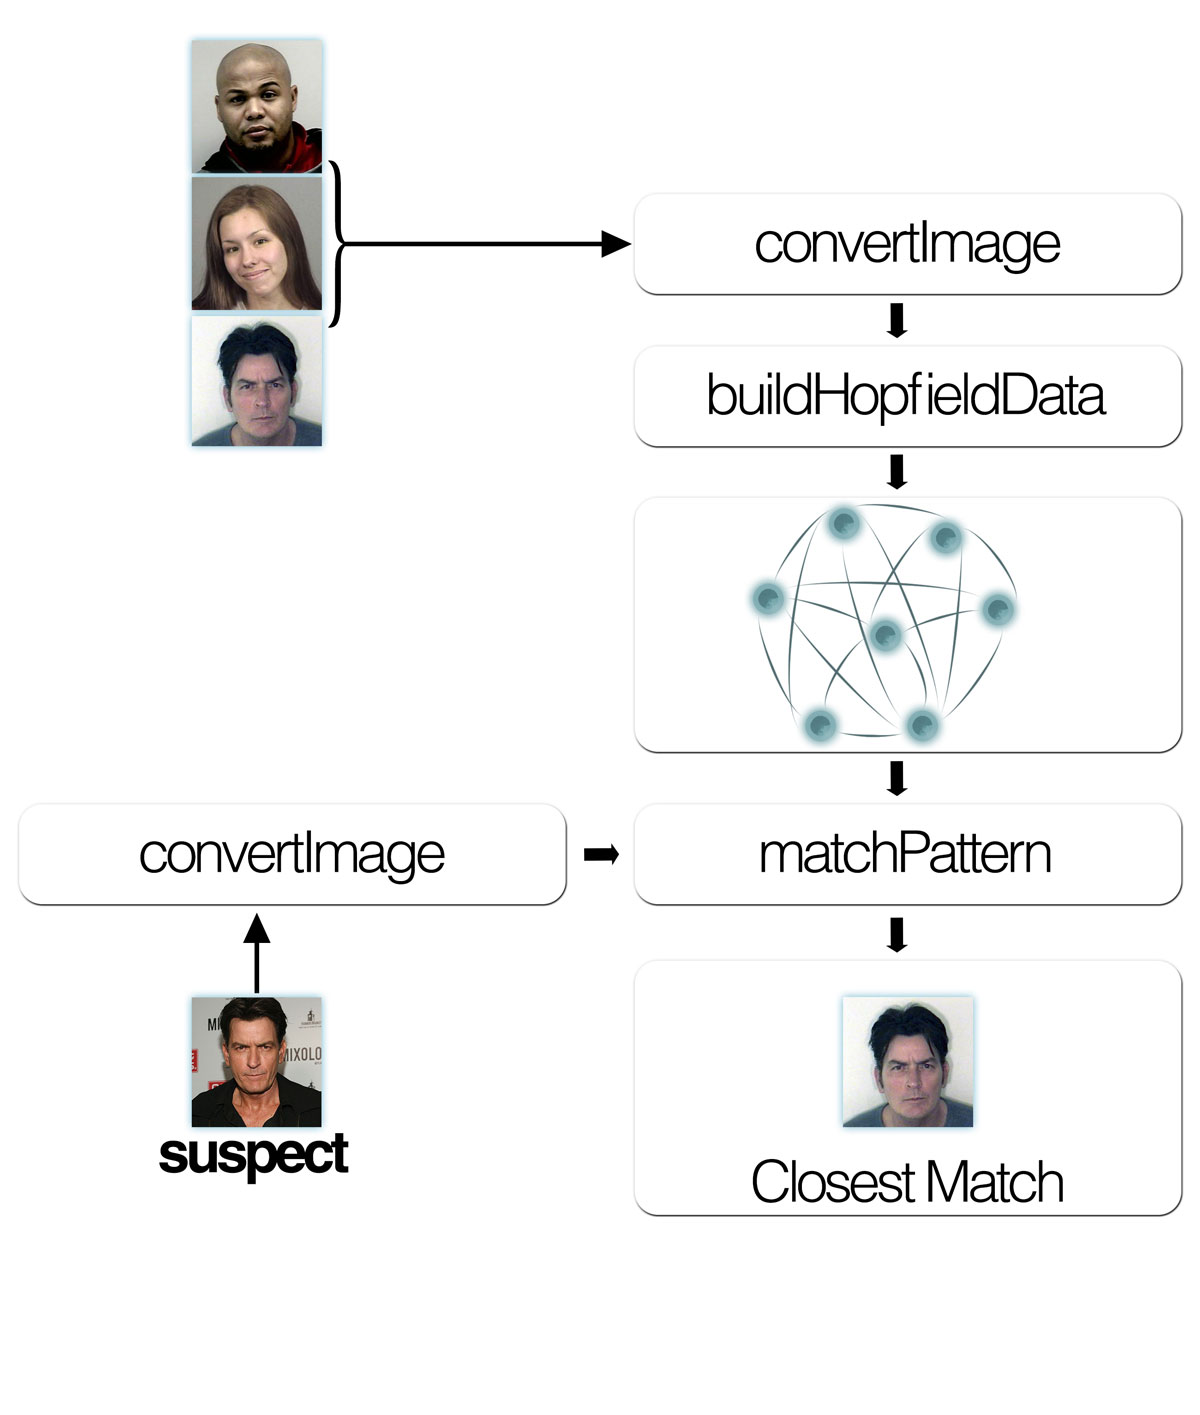
\includegraphics[scale=0.3]{recognition.jpg}
\caption{Outline of the Recognition System demonstrating how the various system components interact}
\label{fig:system}
\end{figure}




\section{Technical Challenges}

\subsection{Computation Time}


\hilight{maybe move detailed discussion to where the algorithm is actually described?}
The common theme of our experiments is measuring and comparing basins of attractions over a multitude of parameters, performed using the Storkey-Valabregue method (see \ref{storkey_basin_size}). As we know, this involves performing a very expensive computation: sampling 100 patterns for each Hamming radius, a maximum of N steps, and for each of those patterns iterative updates are run with the network until convergence is achieved. Though impossible due to properties of Hopfield networks, we can approximate the worst case complexity of the latter as requiring $2^N$ iterations until convergence, $2^N$ being the number of possible states. Thus we may cynically, for the sake of quantifying it, approximate the worst case complexity of the Storkey-Valabregue method to be $O(N2^N)$. While this is probably not an accurate representation of what occurs in practice, it serves to demonstrate the sheer amount of computation performed.

Naturally, this posed a significant computational challenge which we had to be overcome, as we typically obtain a large number of samples of basin measurements for our experiments, in the order of hundreds of samples for a given experiment. One way in which we overcome this limitation is by exploiting parallelism both at the process level (trivially achieved using \textbf{Haskell}!) and at the machine level, running multiple experiments on several lab machines. We also sought to improve the quality of our code itself, using profiling to identify hotspots. \hilight{next subsection on benchmarks}


\subsection{Big Data}

Another challenge which we have faced is dealing with the sheer amount of data generated by our experiments. The data typically needs to be collected, processed, and presented in a consistent manner. In order to address this issue, we attempted to automate such tasks. Automation is key, as it saves time, is not prone to (low level) human error, and generally scales well. Achieving this goal required the joint cooperation of three areas:

\begin{itemize}
\item Experiment executables should output data in a sensible and easy to parse format. Ideally, the output data should not be heavily processed so as to allow flexible use of it.

\item Writing scripts which format and aggregate data, typically calculating the mean value.

\item Presentation of data in the form of graphs of tables ought to be consistent. Ideally, the data should be kept separate from the format or design of its final presentation form. The \texttt{pgfplots} package for \LaTeX was very helpful for this.
\end{itemize}


\section{Anticipated Risks}

\subsection{Failure to match a pattern stored}
One of the risks associated with using the Hopfield model is that the converged pattern may not be one of the stored patterns, but rather a spurious pattern, as explained in section \ref{spurious_patterns}. This poses a problem for our recognition application, which needs to return as a result the closest matched stored pattern. Another issue with similar repercussions is that even after a large number of iterations are run, the pattern has not yet converged.
One solution to this \hilight{have we? also cross ref if applicable} is to simply output the closest stored pattern available. More precisely, the pattern that has the smallest Hamming distance between it and the current state of the system. This makes our image recognition robust to such unfortunate occurrences.


\subsection{A stored pattern not a fixed point}
It is possible that the given set of training patterns are such that some of the patterns simply cannot be ``stored'' in the network, i.e. it is not a fixed point of the network. The probability of this occurring increases as the relative number of training patterns with respect to the number of neurons increases \hilight{cross ref to capacity}.
The best way to deal with this problem is to perform a check (using \texttt{checkFixed}) \hilight{make sure we do that} and, if detected, report it  to the user and allow them to take action. The typical remedy for this would be to increase the number of neurons in the network, at the expense of increased resource usage in both space and time.


\subsection{Floating point calculation}
As we are dealing with extensive calculations of floating point value, we must be careful when dealing with such quantities. In particular, equality comparisons are likely to yield unexpected results. This has had an impact on some tests as well as functions such as \texttt{validWeights}. We have taken care of this problem by replacing equality comparisons and similar with fuzzy equality comparisons, with some accepted margin of error $\epsilon$.


% Chapter 5
% Chapter 5
\chapter{Evaluation}
% Step back and say things like:
% "X worked out well"
% "in hindsight we could have used this tool instead"

% How do we know that our code works?
% e.g. functionality + performance testing
% show relevant testing *results*

% In a nutshell, how successful was this project
% Tony: "DONT SAY: all our objectives (from intro) were met. Have the maturity
% to show your mistakes and more importantly what you learned!"


\section{Implementation}
% In here, we can evaluate our implementation ... Talk about why Haskell was slow for computing the experiments, how we overcame this, ...

\hilight{we need to add some sub-sections here, or bullet points ... this wall of text would only appeal to Chatley}
%why Haskell?
In a nutshell, we are content with the choice of our tools and with our implementation of the neural network. Since our mathematical core of the algorithm does not contain much state information, we chose to implement our project in Haskell.
The strong types allowed us to have confidence in the code we write. Since most of our experiments took a lot of computation time, we had to make sure they run seamlessly and don't crash in the middle of the execution because of a pattern match failure.

There are a lot of advantages in using Haskell, including its clarity and correctness. The type system enforces the programmer to have a clear understanding of the problem and the various solutions available, which leads to high quality code.
Using Haskell came with an initial price: while all the group members were familiar with the language due to our course in first year, we soon realised that we only played with Haskell before. Because of our project, we now deeply appreciate its true beauty and power.

This early overhead turned out to be very small compared to the benefits and the satisfactions we got back. The project enabled us to learn about neural networks and attachment types, but we chose to exploit this opportunity in order to become better using a programming language we like (see fig ~\ref{fig:Haskell Proficieny Index over time}).
\begin{figure}[h]
  \centering1
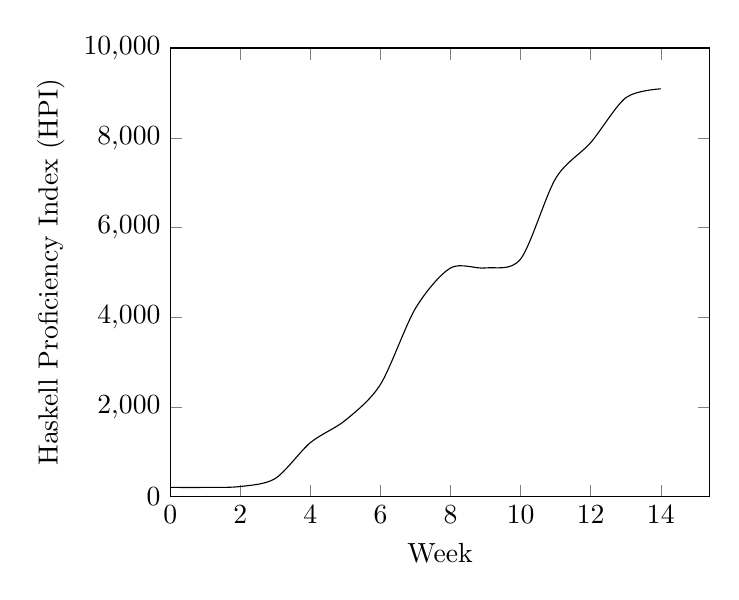
\begin{tikzpicture}
\begin{axis}[
xmin = 0,
ymin = 0,
xlabel = Week,
ylabel = Haskell Proficiency Index (HPI),
scaled y ticks = false,
y tick label style={/pgf/number format/fixed}
]

\addplot [
color = black,
mark = *, % A filled circle
mark = none,
smooth  % draw smooth curve
] coordinates {
(0,200)
(1,200)
(2,220)
(3,400)
(4,1200)
(5,1700)
(6,2500)
(7,4200)
(8,5100)
(9,5100)
(10,5300)
(11,7100)
(12,7900)
(13,8900)
(14,9100)
};

\end{axis}
\end{tikzpicture}

\caption{Average Haskell Proficiency Index over time.}
\label{fig:Haskell Proficieny Index over time}
\end{figure}

\subsection{Optimising for speed}

While testing the recognition application, we realised that our implementation was not as fast as we would have liked it to be, and imposed serious limitation on the size of the networks we were able to try out.
As a consequence, we invested a good amount of time in understanding Haskell compiler optimisations, runtime characteristics, and profiling tools. Using time and allocation profiling, we found that two inner loops in our numerical network updating code were slowing us down significantly. By changing 12 lines to manually unroll the involved list comprehensions into tail-recursive functions we were able to get an overall 4-times speedup of our program.
Additionally, Haskell's being a purely functional programming language allows for easy and efficient parallelism.
By replacing a top-level map with a parallel map function, our program immediately scaled up to the eight processes that were available on the lab machines we used. Because our main processing time is spent in numerical, cache-local loops, we also got almost 8-times improved performance from this. This final scaling success is an improvement over an initial try in which we parallelized an inner loop, which turned out to be too fine-grained.

% already good performance that we achieved through writing code without side effects and ghc's highly optimizing native code generator.

\subsection{Unit Testing}

Unit testing of our Haskell functions was performed using the HUnit framework. This allowed us to heavily test the complex functions responsible for performing updates or calculating energy and capacity, thus making sure that important invariants always hold: energy is always monotonically decreasing, capacity is following the theoretical trends and updates eventually converge to an attractor.

%show some testing results here

\section{Evaluating our experiments}
% We can use this section to evaluate some of our experiments, point out any inconsistencies, limitations, ...



% Chapter 6
\chapter{Conclusion and Future Extensions}
% Tony: "Conclusion is NOT a summary"
% e.g. result that you did not know about

\section{Analogy with Attachment Theory}

The thorough analysis of the attractor neural networks (Hopfield network and Boltzmann machine) has clearly proven their capabilities, being able to model complex attachment types. However, research done in linking the model with the real-life scenario is quite slim, and further work needs to be dedicated especially in this area.

\section{Future Extensions}

We have introduced the reader with only a few flavours of what Attractor neural networks can really do. Deep investigations should be done in order to further investigate their properties, and really push them to the limit. These might provide a good source of inspiration for developing even more biologically realistic models, that better simulate the human brain.

Another line of extension is about providing better visualisation tools for these highly abstract models, that work on N-dimensional spaces. Parallel coordinates can be used for easily visualising the N-dimensional attractors, or the convergence of the network to such an attractor. Furthermore, plots can be done on the available number of neurons that can be updated at each step in the convergence process.

The experiments we did on Hopfield networks should be reproduced using the Restricted Boltzmann machine, which is a more powerful neural network. Furthermore, biological plausibility also needs to be kept in mind, which would surely provide us with more efficient learning systems.

\subsection{Inconsistencies in the results}
\label{inconsistencies}

It is important mentioning a few apparent inconsistencies in the cluster experiments. For examples, the experiments that have been done, using 1 cluster, display inconsistencies in the results between methods T1 and T2. We believe the main reason for this inconsistency is the limitation of the methodology for sampling Gaussian-distributed patterns and the poor use of the state space. Another reason for this apparent inconsistency might also be the presence of spurious attractors, that can interfere with the real attractors and ``steal'' part of their basins.

Another reason for the inconsistencies might also be the chaotic shape of the basins. Since the Storkey-Valabregue measurement is only good for hyper-spherical basin shapes. A more powerful method, such as a Monte Carlo sampling in the neighbourhood, is necessary for measuring basins that don't have hyperspherical shapes.

% Chapter 7
% Chapter 7
\chapter{Project Management}
% Use this to convey your *group collaboration*
% Team organisation, supervisor, software engineering team skills

% DONT give lots of text about the SE process (a la diary), rather your team,
% deliverables, etc

% Note that group collaboration is worth 30%. This is part assessed by our
% supervisor comments, how we present ourselves, and probably a bit will be
% influenced by what we say here. Bare this in mind!


\section{Project Organisation}
%introduction
We started out the project by thoroughly investigating the Hopfield model, reading important research papers that were describing it in detail and showing the potential for other applications.

%allocation of work
Once we had a firm understanding of the mathematical model, we assigned various tasks to each members in order to create a simple image recognition application. Wael and Mihaela started implementing the core algorithm in Haskell, based on information gathered from the research papers. Razvan implemented the image preprocessing in C, while Niklas was integrating the Haskell algorithmic core with the C programs. Lukasz worked on implementing the GUI and image loading, GUI usability and correctness testing, as well as supplying much of the artistic work, including that found throughout this report.

%mention about Chatley
We heavily followed the advice that Dr. Chatley offered in the Software Engineering Lectures. Therefore, we used to have regular weekly meetings and perform iterative development in order to make sure we have a working version of our product at any time.

% we didn't use Agile
Although we did not use any popular software engineering methodology, such as Agile development, we did make sure we are on track with the project requirements. We closely collaborated in order to ensure timely delivery and were flexible to quick changes that came across the progress of the project.


\section{A story}
It is in difficult times that the value of team work really flourishes, as the story of our experiments shall show. As aforementioned, running our experiments posed as a formidable difficulty due the hefty processing time it required. Such experiments would last long hours, sometimes overnight. This was deemed unacceptable to us, and we sought a solution to this problem. Various members of the team collaborated in subgroups, each focusing on a particular aspect of improvement. These sub-groups were not rigid subdivisions of the team, quite the contrary, they were dynamic and self-arranging. One task undertaken by a subgroup is the optimisation of the experiment, in particular those arising from running the Storkey-Valabregue method. Iteratively optimising the code and testing the results locally and at scale (by actually running the experiments). Another subgroup worked on exploiting the resources available to us, developing the code and writing scripts to parallelize the experiments to run on multiple cores and multiple machines. Eventually, the experiments exhibited an improvement of at least 30 fold for some experiments (the magic of parallelism!). So what can we conclude from this? Team work can perform miracles!


\nocite{*} % Show all Bib-entries
\bibliographystyle{plain}
\bibliography{main}



\chapter{Appendices}

%%%%%%%%%% Start TeXmacs macros
\newcommand{\mathpi}{\pi}
\newcommand{\nin}{\not\in}
\newcommand{\nosymbol}{}
\newcommand{\tmem}[1]{{\em #1\/}}
\newcommand{\tmkbd}[1]{\texttt{#1}}
\newcommand{\tmfloatcontents}{}
\newlength{\tmfloatwidth}
\newcommand{\tmfloat}[5]{
  \renewcommand{\tmfloatcontents}{#4}
  \setlength{\tmfloatwidth}{\widthof{\tmfloatcontents}+1in}
  \ifthenelse{\equal{#2}{small}}
    {\ifthenelse{\lengthtest{\tmfloatwidth > \linewidth}}
      {\setlength{\tmfloatwidth}{\linewidth}}{}}
    {\setlength{\tmfloatwidth}{\linewidth}}
  \begin{minipage}[#1]{\tmfloatwidth}
    \begin{center}
      \tmfloatcontents
      \captionof{#3}{#5}
    \end{center}
  \end{minipage}}
%%%%%%%%%% End TeXmacs macros


\chapter{Errors in Hopfield networks}

When a Hopfield network is trained using a list of patterns, it is desired
that those patterns are attractors, which requires that they are fixed points.
In case one of the patterns is not a fixed point, it is said that the network
has an error.

We will now derive the equations for errors in Hopfield networks.
Firstly, we shall derive the probability of error for a pattern which was used
for training, given that all the patterns were independent. Secondly, we will
derive the equation of error for a super attractor: a pattern which was used
to train the network, but which appeared in the training multiple times. The
assumption for this derivation is that the other training patterns are
independent. In the context of attachment types, we can assume that the super
attractor is the primary care giver, which was consistent in his/her
behaviour, and that the other encounters of the child were independent.

\section{Stability of stored states, given independence of all stored
patterns}

Consider a pattern stored in the network \tmtextit{x$^k$}. We want to find out
the probability of error for that pattern: how probable is that given that
\tmtextit{x$^k$} is stored in the network it is not a fixed point?

Given the update formulae for neuron $i$ in pattern \tmtextit{k } $\left( 1
\left) \right. \right.$ and the formulae for the weights, according to the
training of the network ($2$):
\[ h_i^k = \sum^N_{j = 1} w_{i j} x_j^k  \]

\begin{equation}
  w_{\tmop{ij}} = \frac{1}{N} \sum^p_{l = 1} x^l_{i^{}} x_j^l
\end{equation}
we obtain by substitution:
\[ h_i^k = \sum^N_{j = 1} \left(^{} \frac{1}{N} \sum^p_{l = 1} x^l_{i^{}}
   x^l_j \right)_{} \cdot x_j^k = \frac{1}{N}  \sum^N_{j = 1} \sum^p_{l = 1}
   x^l_{i^{}} x^l_j x^k_{^{} j} = \]
\[ = \frac{1}{N}  \sum^N_{j = 1} x^k_{i} x^k_j x^k_{^{j}} \noplus
   \noplus + \frac{1}{N}  \sum^N_{j = 1} \sum^p_{l = 1 \nocomma, l \neq k}
   x^l_{i^{}} x^l_j x^k_{^{} j} \]
\[ = \frac{1}{N}  \sum^N_{j = 1} x^k_{i} + \frac{1}{N}  \sum^N_{j = 1}
   \sum^p_{l = 1 \nocomma, l \neq k} x^l_{i} x^l_{j} x^k_{j} = x^k_{i}
   + \frac{1}{N}  \sum^N_{j = 1} \sum^p_{l = 1 \nocomma, l \neq k} x^l_{i}
   x^l_{j} x^k_{j} \]
\[  \]
$\tmop{The} \tmop{new} \tmop{value} \tmop{of}$ neuron i $x^{k'}_i $is given by
the sign of $h_i^k $, so:




\begin{equation}
  h^k_i x^k_i \left\{ \begin{array}{l}
    \geqslant 0 \nocomma \nocomma \nocomma \tmop{if} x^k_{i'} = x^k_i\\
    < 0 \tmop{otherwise}
  \end{array} \right.^{}_{} \Rightarrow -_{} h^k_i x^k_i \left\{
  \begin{array}{l}
    \leqslant 0 \nocomma \nocomma \nocomma \tmop{if} x^k_{i'} = x^k_i\\
    > 0 \tmop{otherwise}
  \end{array} \right.
\end{equation}
\begin{equation}
  - h^k_i x^k_{^{} i} = - x^k_{i^{}} x^k_{i^{}} - x^k_{i^{}} \cdot \left(
  \frac{1}{N}  \sum^N_{j = 1} \sum^p_{l = 1 \nocomma, l \neq k} x^l_{i^{}}
  x^l_j x^k_{^{} j} \right) = 1 \begin{array}{c}
    - \underbrace{\frac{1}{N} \sum^N_{j = 1} \sum^p_{l = 1 \nocomma, l \neq k}
    x^l_{i^{}} x^l_j x^k_{^{} j} x^k_i}_{C^k_i}
  \end{array}
\end{equation}
\ \ \ \ \ \ \ \ \ \ \ \ \ \ \ \ \ \ \ \ \ \ \ \ \ \ \ \ \ \ \ \ \ \ \ \ \ \ \
\ \ \ \ \ \ \ \ \ \ \ \ \ \ \ \ \ \ \ \ \ \ \ \ \ \ \ \ \ \ \ \ \ \ \ \ \ \ \
\ \ \ \ \ \ \ \ \ \ \ \ \ \ \ \ \ \

From (3) and (4) we conclude that we get an error if $C_i^k > 1$ , so the
probability of getting an error is the given by the probability of \ $C_i^k >
1$.

We model $C_i^k $ as follows. Each $x^l_{i^{}} x^l_j x^k_{^{} j} x^k$ can be
modelled as a sample drawn from a random variable X with $\tmop{E (X) = 0}$
and $\tmop{Var} (X) = E (x^2) - E (x)^2 = 1.0$

By using the central limit theorem and by approximating $N \left( p \right.$ -
$1$) to $Np$ :
\[ \frac{1}{Np} \sum_{i = 1}^{Np} X_i \sim N \left( 0 \nocomma, \frac{1}{N p}
   \right) \]


Thus,
\[ \frac{1}{N} \sum_{i = 1}^{Np} X_i \sim N \left( 0 \nocomma, \frac{p}{N}
   \right) \]
\[ C^k_i \sim N \left( 0 \nocomma, \frac{p}{N} \right) \]
By denoting $\frac{p}{N}$ with $\sigma :$
\[ P \left( C^k_i > 1 \right) \simeq \frac{1}{\sqrt{2 \mathpi} \sigma}
   \int^{\infty}_1 e^{- \frac{x^2}{2 \sigma^2}} \tmop{dx} = \frac{1}{\sqrt{2
   \mathpi} \sigma} \int^{\infty}_{\frac{1}{\sqrt{2} \sigma}} e^{- y^2}
   \sqrt{2} \sigma \tmop{dy} = \]
\[ = \frac{1}{\sqrt{\mathpi}} \int^{\infty}_{\frac{1}{\sqrt{2} \sigma}} e^{-
   y^2} \tmop{dy} = \frac{1}{\sqrt{\mathpi}} \left( \int^{\infty}_0 e^{- y^2}
   \tmop{dy} - \int^{\frac{1}{\sqrt{2} \sigma}}_0 e^{- y^2} \tmop{dy} \right)
   = \]
\[ = \frac{1}{\sqrt{\mathpi}} \int^{\infty}_0 e^{- y^2} \tmop{dy} -
   \frac{1}{\sqrt{\mathpi}} \int^{\frac{1}{\sqrt{2} \sigma}}_0 e^{- y^2}
   \tmop{dy} = \frac{1}{\sqrt{\mathpi}} \ast \frac{\sqrt{\pi}}{2} \noplus -
   \frac{1}{2} \tmop{erf} \left( \frac{1}{\sqrt{2 \sigma}} \right) = \]
\[ = \frac{1}{2} \left( 1 \noplus \noplus - \tmop{erf} \left( \frac{1}{\sqrt{2
   \sigma}} \right) \right) = \frac{1}{2} \left( 1 \noplus \noplus -
   \tmtextit{\tmop{erf}} \left( \sqrt{\frac{N}{2 p}} \right) \right)  \]
\[ \tmop{where} \tmop{err} x = \frac{1}{\sqrt{2 \pi}} \int^x_0 e^{- x^2
   }_{^{^{}}} \tmop{dx} \]

\[  \]
\[  \]
\section{Stability of a super attractor, given independence of all other
stored patterns}



By following the above way of reasoning, we compute the probability of error
for a super attractor.

Given that the super attractor has degree d (it appears d times in the list of
patterns used to train the network), we compute the probability that it is not
a fixed point.

Let $x^k_{}$ be the supper attractor with degree d.

Let S = $\left\{ i \left|  \right. \right. x^i_{} = x^k$ , i {\tmem{$\in
\left\{ 1 \ldots p \right\} $}}\}, be the set of indexes of occurrences of the
supper attractor $x^k_{}$.

$\tmop{We} \tmop{assumed} \tmop{that} \tmop{the} \tmop{super} \tmop{attractor}
\tmop{has} \tmop{degree} d \nocomma \nocomma \nocomma \Rightarrow \left| S
\left| = d \nosymbol \right. \right.$.


\[ h_i^k = \sum^N_{j = 1} \left(^{} \frac{1}{N} \sum^p_{l = 1} x^l_{i^{}}
   x^l_j \right)_{} \cdot x_j^k = \frac{1}{N}  \sum^N_{j = 1} \sum^p_{l = 1}
   x^l_{i^{}} x^l_j x^k_{^{} j} = \]
\begin{eqnarray*}
  \frac{1}{N}  \sum^N_{j = 1} \sum_{l \in S}^p x^k_{i} x^k_j x^l_{j} \noplus \noplus + \frac{1}{N}  \sum^N_{j = 1} \sum^p_{l \nin S}
  x^l_{i} x^l_j x^k_{j}  & = &  \frac{1}{N}  \sum^N_{j = 1} \sum_{l
  \in S}^p x^k_{i} x^k_j x^k_{j} \noplus \noplus + \frac{1}{N}
  \sum^N_{j = 1} \sum^p_{l \nin S} x^l_{i} x^l_j x^k_{j} =\\
  &  & \\
  \frac{1}{N}  \sum^N_{j = 1} \sum_{l \in S}^p x^k_{i} \noplus + \noplus
  \frac{1}{N}  \sum^N_{j = 1} \sum^p_{l \nin S} x^l_{i} x^l_j x^k_{j}
  & = &  \frac{1}{N} N d x^k_{i} \noplus + \frac{1}{N}  \sum^N_{j =
  1} \sum^p_{l \nin S} x^l_{i} x^l_j x^k_{j} =
\end{eqnarray*}
\[ = d x^k_{i^{}} \noplus + \frac{1}{N}  \sum^N_{j = 1} \sum^p_{l \nin S}
   x^l_{i^{}} x^l_j x^k_{^{} j} \]
Thus
\[ - h^k_i x^k_i = - d x_i^k x_i^k - \frac{1}{N}  \sum^N_{j = 1} \sum^p_{l
   \nin S} x^l_{i^{}} x^l_j x^k_{^{} j} x^k_{i^{}} = \]
\[ - d - \underbrace{ \frac{1}{N}  \sum^N_{j = 1} \sum^p_{l \nin S} x^l_{i^{}}
   x^l_j x^k_{^{} j} x^k_{i^{}} }_{S^k_i} \]
\ \ \ \ \ \ \ \ \ \ \ \ \ \ \ \ \ \ \ \ \ \ \ \ \ \ \ \ \ \ \ \ \ \ \ \ \ \ \
\ \ \ \ \ \ \ \ \ \ \ \ \ \ \ \ \ \ \ \ \ \ \

In order to get an error, $\tmop{minus} h^k_i x^k_i \leqslant 0 \nocomma$ ,
so $S^k_i$ $\geqslant d \nosymbol$. By using the same reasoning as before,
\[ \frac{1}{N \left( p - d \right)} \sum_{i = 1}^{N \left( p - d \right)} X_i
   \sim N \left( 0 \nocomma, \frac{1}{N \left( p - d \right)} \right) \]
\[ \frac{1}{N} \sum_{i = 1}^{N \left( p - d \right)} X_i \sim N \left( 0
   \nocomma, \frac{p - d}{N} \right) \]
\[ S^k_i \sim N \left( 0 \nocomma, \frac{p - d}{N} \right) \]
By denoting $\frac{p - d}{N}$ with $\sigma :$
\[ P \left( S^k_i > d \right) \simeq \frac{1}{\sqrt{2 \mathpi} \sigma}
   \int^{\infty}_d e^{- \frac{x^2}{2 \sigma^2}} \tmop{dx} = \frac{1}{\sqrt{2
   \mathpi} \sigma} \int^{\infty}_{\frac{d}{\sqrt{2} \sigma}} e^{- y^2}
   \sqrt{2} \sigma \tmop{dy} = \]
\[ = \frac{1}{\sqrt{\mathpi}} \int^{\infty}_{\frac{d}{\sqrt{2} \sigma}} e^{-
   y^2} \tmop{dy} = \frac{1}{\sqrt{\mathpi}} \left( \int^{\infty}_0 e^{- y^2}
   \tmop{dy} - \int^{\frac{d}{\sqrt{2} \sigma}}_0 e^{- y^2} \tmop{dy} \right)
   = \]
\[ = \frac{1}{\sqrt{\mathpi}} \int^{\infty}_0 e^{- y^2} \tmop{dy} -
   \frac{1}{\sqrt{\mathpi}} \int^{\frac{d}{\sqrt{2} \sigma}}_0 e^{- y^2}
   \tmop{dy} = \frac{1}{\sqrt{\mathpi}}  \frac{\sqrt{\pi}}{2} \noplus -
   \frac{1}{2} \tmop{erf} \left( \frac{d}{\sqrt{2 \sigma}} \right) = \]
\[ = \frac{1}{2} \left( 1 \noplus \noplus - \tmop{erf} \left( \frac{1}{\sqrt{2
   \sigma}} \right) \right) = \frac{1}{2} \left( 1 \noplus \noplus -
   \tmtextit{\tmop{erf}} \left( \sqrt{\frac{N}{2 \left( p - d \right)}}
   \right) \right)  \]


\section{Computing network parameters given maximum accepted error}

Assuming all training patterns are independent, we can use the above results
to determine the minimum number of neurons which should be used for the
network given the number of training patterns we want to store. In the case of
image recognition, this can provide to be useful as it can give a guideline
towards how to resize the images in order to bring them to the same size
(patterns which are stored in a Hopfield network need to have equal lengths).
It also enables us to compute the capacity of a network of given size, in
order to minimise errors.

Given p and N, we deduced the probability of error for the network. Thus,
conversely, we can compute the maximum ratio of p and N to ensure that the
probability of error does not exceed a maximum accepted error probability.
\[ P_{\tmop{error}} = \frac{1}{2}  \left( 1 \noplus \noplus -
   \tmtextit{\tmop{erf}} \left( \sqrt{\frac{N}{2 p}} \right) \right)  \]
\begin{eqnarray*}
  \Rightarrow \tmop{erf} \sqrt{\frac{N}{2 p}} = 1 - 2 P_{\tmop{error}} &
  \Rightarrow & \sqrt{\frac{N}{2 p}} = \tmop{inverf} \left( 1 - 2
  P_{\tmop{error}} \right)
\end{eqnarray*}
\[ \Rightarrow \frac{N}{p} = 2 \left( \tmop{inverf} \left( 1 - 2
   P_{\tmop{error}} \right) \right)^2 \]
\begin{eqnarray*}
  \frac{p}{N} = \frac{1}{2 \left( \tmop{inverf} \left( 1 - 2 P_{\tmop{error}}
  \right) \right)^2} & \tmop{and} & N = 2 p \left( \tmop{inverf} \left( 1 - 2
  P_{\tmop{error}} \right) \right)^2
\end{eqnarray*}
where inverf is the inverse of the erf function.

\section{Measurements using the error of a network for independent
patterns}

We will now give the reader an idea of how one should accommodate a fixed
number of patterns depending on the error accepted by the application, by
creating networks of appropriate size.

\ \ \ \ \ \ \ \ \ \ \ \ \ \ \ \ \ \ \ \ \ \ \ \ \ \ \ \ \ \

\begin{table}[h]
\centering
  \begin{tabular}{|c|c|c|}
    \hline
    \tmtextbf{p} & \tmtextbf{error} & \tmtextbf{N}\\
    \hline
    100 & 0.1 & 165\\
    \hline
    100 & 0.01 & 542\\
    \hline
    100 & 0.05 & 271\\
    \hline
    100 & 0.001 & 955\\
    \hline
  \end{tabular}
  \caption{Getting the minimum numbers of neurons required by the network by
  fixing the error and the number of patterns used to train the network.}
\end{table}

The following table describes the capacity of the network in terms of the
error accepted, by fixing the size of the network.

\begin{table}[h]
  \centering
  \begin{tabular}{|c|c|c|}
    \hline
    \tmtextbf{N} & \tmtextbf{error} & \tmtextbf{p}\\
    \hline
    1000 & 0.1 & 608\\
    \hline
    1000 & 0.01 & 184\\
    \hline
    1000 & 0.05 & 359\\
    \hline
    1000 & 0.001 & 104\\
    \hline
  \end{tabular}\tmtextbf{}
  \caption{Getting the capacity of a network by fixing the error and the size
  of a network.}
\end{table}

The above results can be reproduced by using the Analysis module. For example,
by using \tmtexttt{ghci}:

{\tmkbd{\tmtexttt{}*Analysis > computeErrorSuperAttractor 10 100}}

The first argument of the function is $p$ (the number of training patterns),
and the second one is $N$ (the size of the network). A similar function can be
used for a given network \tmtexttt{computeErrorSuperAttractor}, that given a
network computes the probability of error of the super attractor. The caller
has to ensure that training patterns are independent in order for the
computation to be correct.

\section{Decreasing the error by using one super attractor}

Above we described the derivation for obtaining the error of a super
attractor, given its degree. We remind the reader that we did this under the
assumption that all other training patterns are independent. We will now show
how the error of a pattern decreases if it is made a super attractor, by
varying the number of times it is presented to the network during training.

\begin{table}[h]
\centering
\begin{tabular}{|c|c|c|c|}
  \hline
  \tmtextbf{degree} & \tmtextbf{p} & \tmtextbf{N} & \tmtextbf{error}\\
  \hline
  1 & 20 & 100 & 1.08 *$10^{- 2}$\\
  \hline
  2 & 20 & 100 & 7.64*$10^{- 3}$\\
  \hline
  5 & 20 & 100 & 4.91*$10^{- 3}$\\
  \hline
  8 & 20 & 100 & $1.95 \ast 10^{- 3}$\\
  \hline
  11 & 20 & 100 & $4.29 \ast 10^{- 4}$\\
  \hline
  15 & 20 & 100 & $3.87 \ast 10^{- 6}$\\
  \hline
\end{tabular}{}

\centering
\begin{tabular}{|c|c|c|c|}
  \hline
  \tmtextbf{degree} & \tmtextbf{p} & \tmtextbf{N} & \tmtextbf{error}\\
  \hline
  1 & 50 & 100 & $7.65 \ast 10^{^{- 2}}$\\
  \hline
  5 & 50 & 100 & 6.80*$10^{- 2}$\\
  \hline
  10 & 50 & 100 & 5.69*10$^{- 2}$\\
  \hline
  20 & 50 & 100 & 3.39*$10^{- 2}$\\
  \hline
  30 & 50 & 100 & $1.26 \ast 10^{- 2}$\\
  \hline
  40 & 50 & 100 & $7.82 \ast 10^{- 4}$\\
  \hline
\end{tabular}{}
\caption{Computing the network error when using a super attractor}
\end{table}

Note that in the second table we are intentionally stressing the network so
that we can notice how super attractors also affect the capacity of the
network.

The above results can be reproduced by using the Analysis module. For example,
by using \tmtexttt{ghci}:

{\tmkbd{\tmtexttt{}*Analysis > computeErrorSuperAttractorNumbers 40 50 100}}

The first argument of the function is the degree of the attractor, the second
one is $p$ and the third one is $N$. A similar function can be used for a
given network \tmtexttt{computeErrorSuperAttractor}, that given a network
computes the probability of error of the super attractor. The caller of the
function has to ensure that the training patterns contain a super attractor
and that the other patterns are independent.

% these do NOT count as part of the suggested page count
% This is probably a good place to explain the models in some detail for example


\end{document}
